\documentclass{article}
\usepackage[utf8]{inputenc}
\usepackage{amsmath, amssymb}
\usepackage{hyperref, float}
\usepackage{booktabs}
\usepackage{pdflscape}
\usepackage{caption, subcaption}
\usepackage{graphicx}
        
\usepackage[preprint]{nips_2018}


\title{San Diego Calibration Results}
\author{Sharad Vikram}
\date{\today}

\begin{document}

\maketitle

\section{Data}

We have been collecting data from nine boards
from three sites in southern California.
\begin{enumerate}
    \item El Cajon
    \item Donovan
    \item Shafter
\end{enumerate}
We have split up the boards and rotated the boards
between locations every two weeks (see \autoref{tab:board-rotations}).

\begin{table}[H]
\centering
\begin{tabular}{l|lll}
                  & \textbf{Round 1} & \textbf{Round 2} & \textbf{Round 3} \\ \hline
\textbf{Board 17} & N/A & El Cajon         & Shafter          \\
\textbf{Board 19} & Donovan          & El Cajon         & Shafter          \\
\textbf{Board 21} & Donovan          & El Cajon         & Shafter          \\ \hline
\textbf{Board 11} & El Cajon         & Shafter          & Donovan          \\
\textbf{Board 12} & El Cajon         & Shafter          & Donovan          \\
\textbf{Board 13} & El Cajon         & Shafter          & Donovan          \\ \hline
\textbf{Board 15} & Shafter          & Donovan          & El Cajon         \\
\textbf{Board 18} & Shafter          & Donovan          & El Cajon         \\
\textbf{Board 20} & N/A & Donovan          & El Cajon        
\end{tabular}
\caption{Board locations for each round}
\label{tab:board-rotations}
\end{table}

We do not have CO data for Shafter and Donovan, so we will focus only on
O3 and NO2.

\section{Distributions}
In this section, we describe
and visualize the distributions
of various values in the data.

\subsection{Environment}

\begin{figure}[H]
\centering
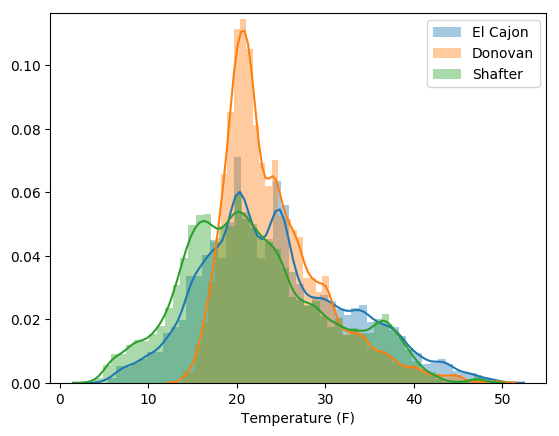
\includegraphics[width=0.5\textwidth]{results/distributions/temperature.png}
\caption{Temperature distribution based on
location}
\label{fig:temperature}
\end{figure}

\begin{figure}[H]
\centering
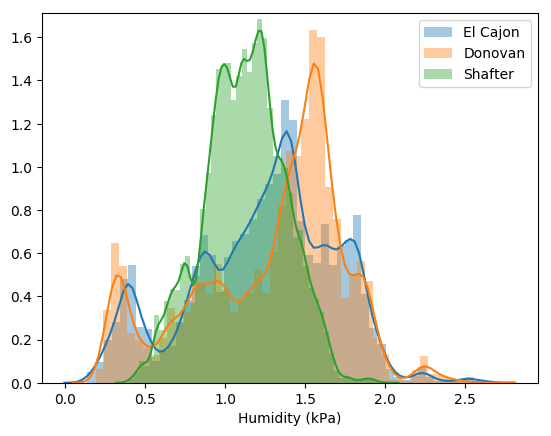
\includegraphics[width=0.5\textwidth]{results/distributions/humidity.png}
\caption{Absolute humidity distribution based on
location}
\label{fig:humidity}
\end{figure}

\begin{figure}[H]
\centering
\begin{subfigure}{0.32\textwidth}
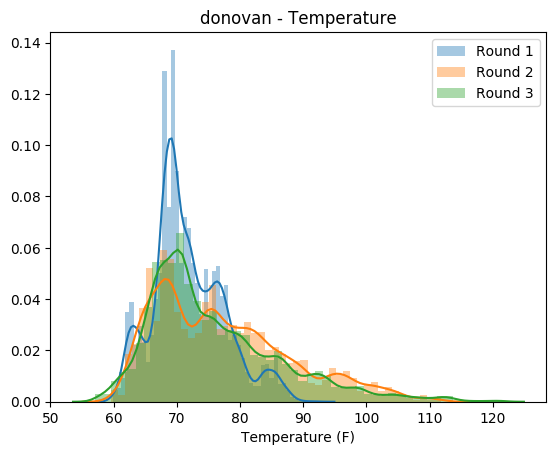
\includegraphics[width=\textwidth]{results/distributions/location_donovan_temperature.png}
\caption{Donovan}
\end{subfigure}
\begin{subfigure}{0.32\textwidth}
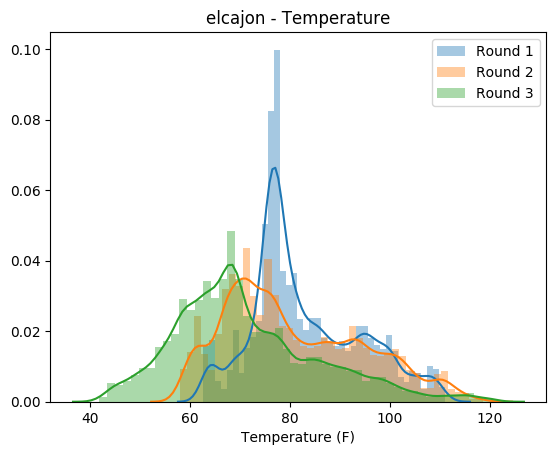
\includegraphics[width=\textwidth]{results/distributions/location_elcajon_temperature.png}
\caption{El Cajon}
\end{subfigure}
\begin{subfigure}{0.32\textwidth}
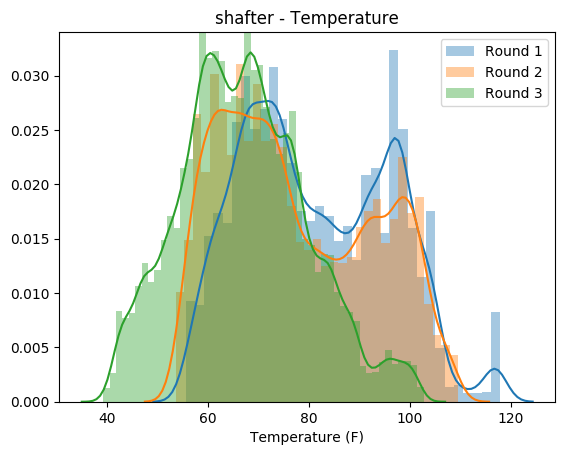
\includegraphics[width=\textwidth]{results/distributions/location_shafter_temperature.png}
\caption{Shafter}
\end{subfigure}
\caption{Temperature at locations}
\label{fig:temperature-locations}
\end{figure}

\begin{figure}[H]
\centering
\begin{subfigure}{0.32\textwidth}
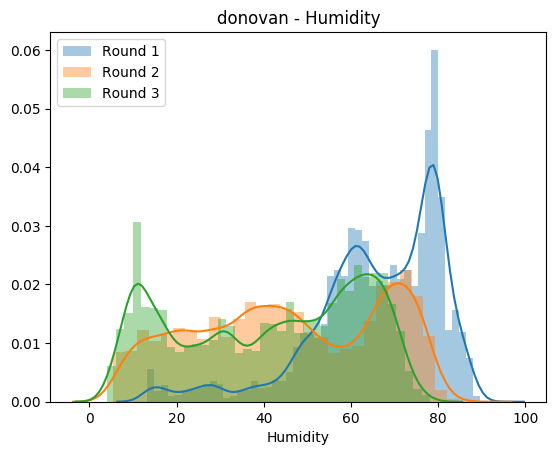
\includegraphics[width=\textwidth]{results/distributions/location_donovan_humidity.png}
\caption{Donovan}
\end{subfigure}
\begin{subfigure}{0.32\textwidth}
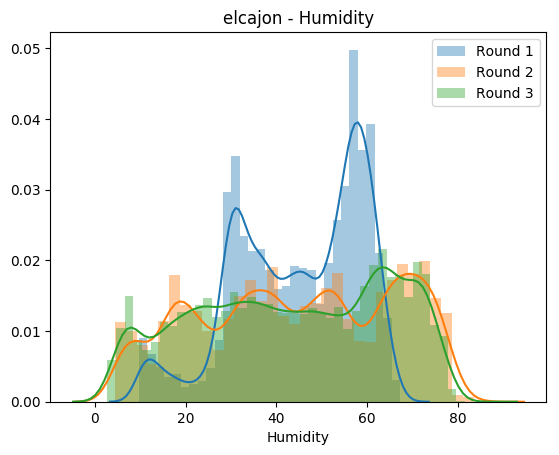
\includegraphics[width=\textwidth]{results/distributions/location_elcajon_humidity.png}
\caption{El Cajon}
\end{subfigure}
\begin{subfigure}{0.32\textwidth}
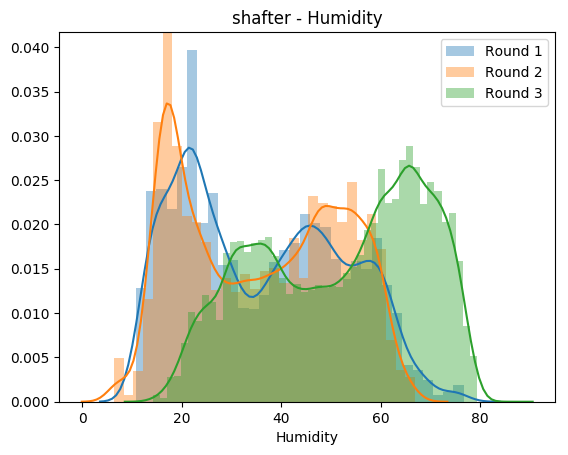
\includegraphics[width=\textwidth]{results/distributions/location_shafter_humidity.png}
\caption{Shafter}
\end{subfigure}
\caption{Humidity at locations}
\label{fig:humidity-locations}
\end{figure}

\begin{figure}[H]
\centering
\begin{subfigure}{0.32\textwidth}
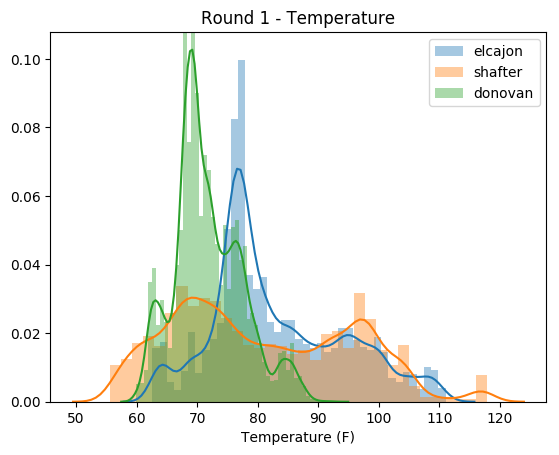
\includegraphics[width=\textwidth]{results/distributions/round1_temperature.png}
\caption{Round 1}
\end{subfigure}
\begin{subfigure}{0.32\textwidth}
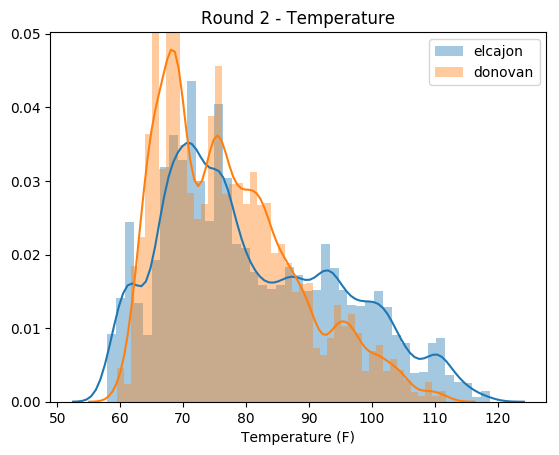
\includegraphics[width=\textwidth]{results/distributions/round2_temperature.png}
\caption{Round 2}
\end{subfigure}
\begin{subfigure}{0.32\textwidth}
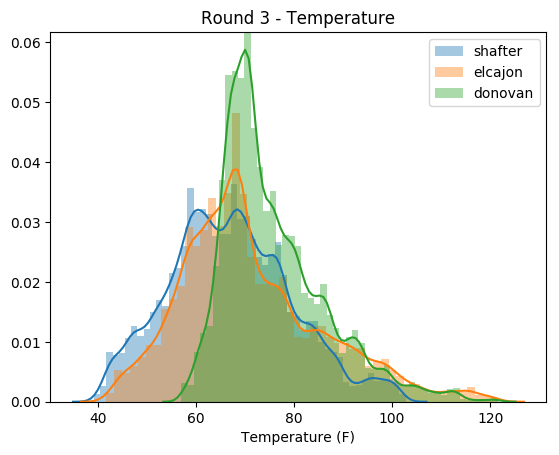
\includegraphics[width=\textwidth]{results/distributions/round3_temperature.png}
\caption{Round 3}
\end{subfigure}
\caption{Temperature over rounds}
\label{fig:temperature-rounds}
\end{figure}

\subsection{Pollutant values}

\begin{figure}[H]
\centering
\begin{subfigure}{0.32\textwidth}
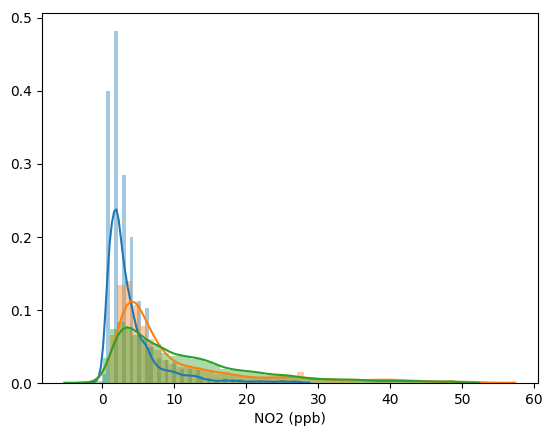
\includegraphics[width=\textwidth]{results/distributions/location_donovan_no2.png}
\caption{Round 1}
\end{subfigure}
\begin{subfigure}{0.32\textwidth}
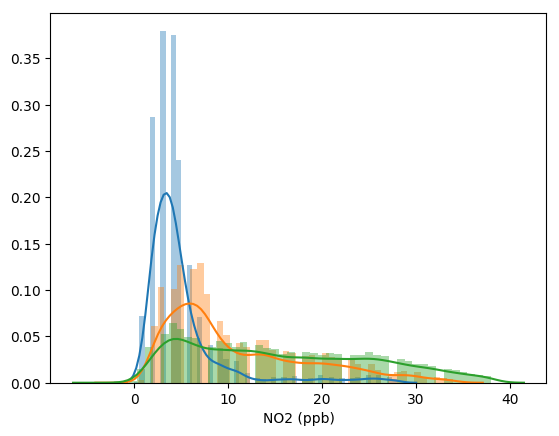
\includegraphics[width=\textwidth]{results/distributions/location_elcajon_no2.png}
\caption{Round 2}
\end{subfigure}
\begin{subfigure}{0.32\textwidth}
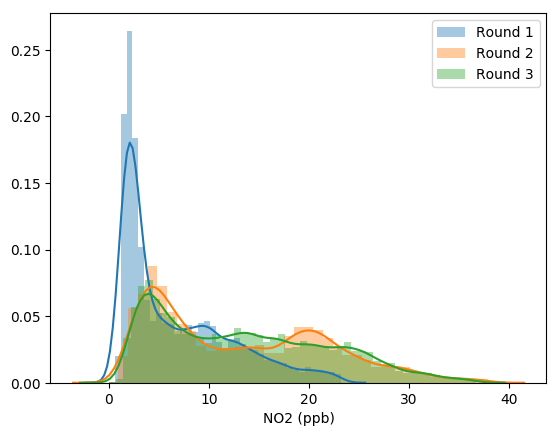
\includegraphics[width=\textwidth]{results/distributions/location_shafter_no2.png}
\caption{Round 3}
\end{subfigure}
\caption{NO2 at locations}
\label{fig:no2-locations}
\end{figure}

\begin{figure}[H]
\centering
\begin{subfigure}{0.32\textwidth}
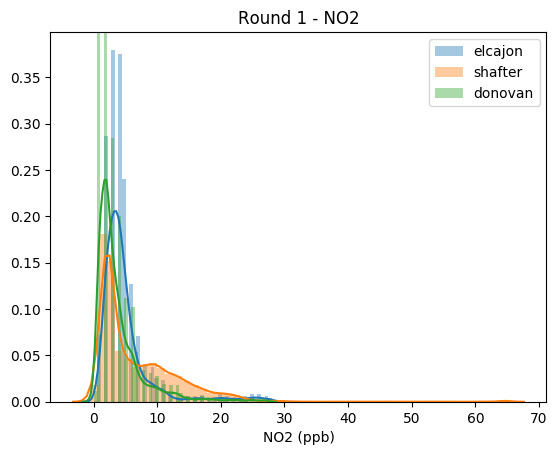
\includegraphics[width=\textwidth]{results/distributions/round1_no2.png}
\caption{Round 1}
\end{subfigure}
\begin{subfigure}{0.32\textwidth}
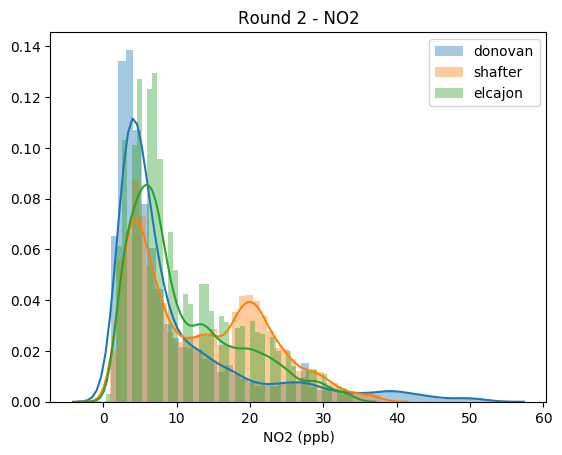
\includegraphics[width=\textwidth]{results/distributions/round2_no2.png}
\caption{Round 2}
\end{subfigure}
\begin{subfigure}{0.32\textwidth}
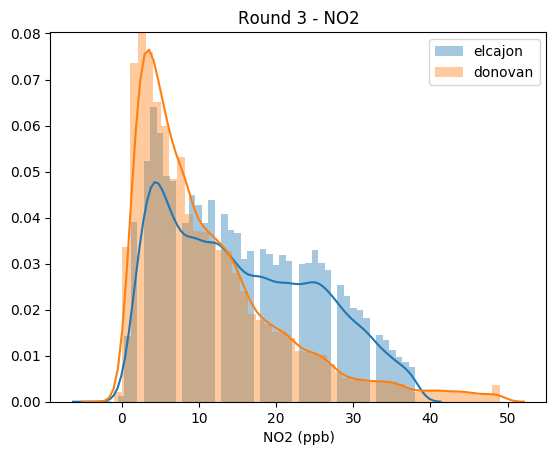
\includegraphics[width=\textwidth]{results/distributions/round3_no2.png}
\caption{Round 3}
\end{subfigure}
\caption{NO2 over rounds}
\label{fig:no2-rounds}
\end{figure}

\begin{figure}[H]
\centering
\begin{subfigure}{0.32\textwidth}
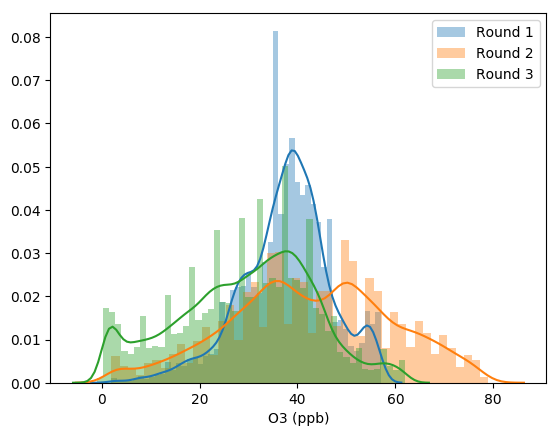
\includegraphics[width=\textwidth]{results/distributions/location_donovan_o3.png}
\caption{Round 1}
\end{subfigure}
\begin{subfigure}{0.32\textwidth}
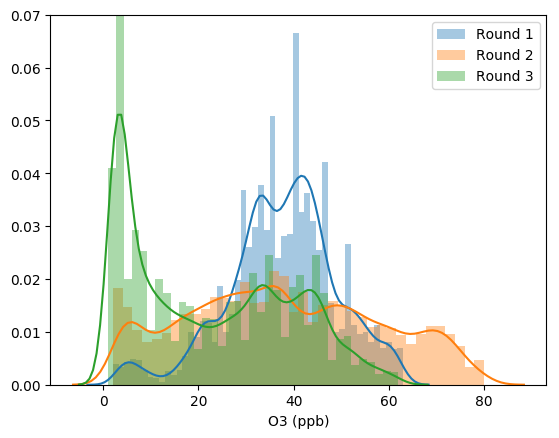
\includegraphics[width=\textwidth]{results/distributions/location_elcajon_o3.png}
\caption{Round 2}
\end{subfigure}
\begin{subfigure}{0.32\textwidth}
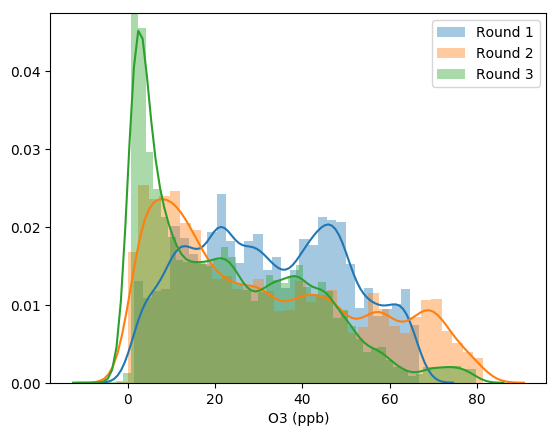
\includegraphics[width=\textwidth]{results/distributions/location_shafter_o3.png}
\caption{Round 3}
\end{subfigure}
\caption{O3 at locations}
\label{fig:o3-locations}
\end{figure}

\begin{figure}[H]
\centering
\begin{subfigure}{0.32\textwidth}
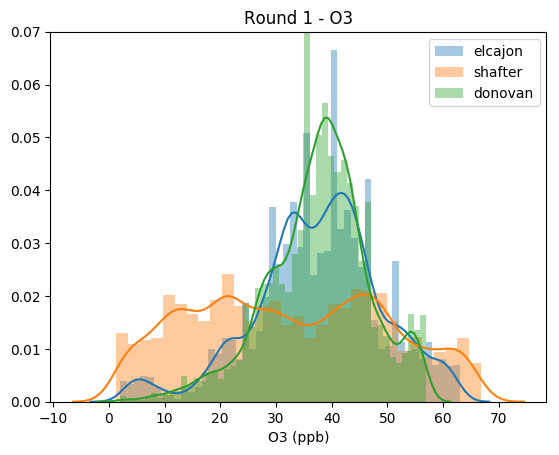
\includegraphics[width=\textwidth]{results/distributions/round1_o3.png}
\caption{Round 1}
\end{subfigure}
\begin{subfigure}{0.32\textwidth}
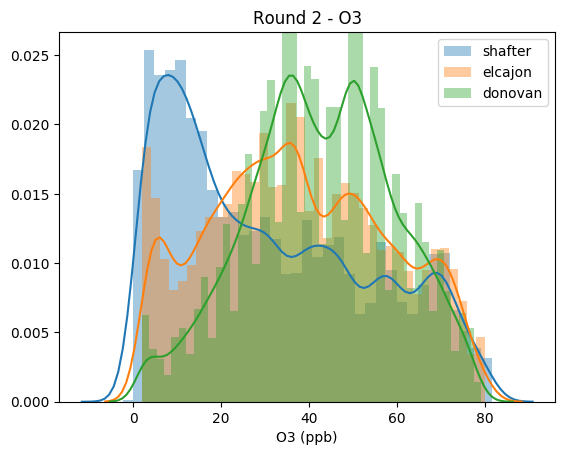
\includegraphics[width=\textwidth]{results/distributions/round2_o3.png}
\caption{Round 2}
\end{subfigure}
\begin{subfigure}{0.32\textwidth}
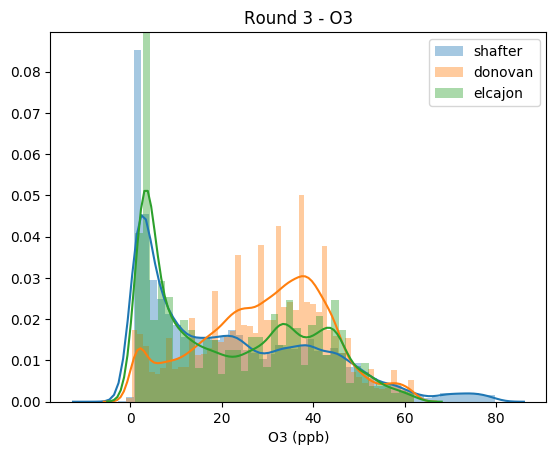
\includegraphics[width=\textwidth]{results/distributions/round3_o3.png}
\caption{Round 3}
\end{subfigure}
\caption{O3 over rounds}
\label{fig:o3-rounds}
\end{figure}


\section{Basic calibration results}

A calibration model takes in sensor readings and environment
variables and outputs pollutant levels. In this basic setup,
we train a model for each board.
We aim to train models that are robust after moving location.

\begin{table}[H]
\centering
\begin{tabular}{|l|l|}
\hline
\textbf{Level 0} & Train on location A and test on location A \\ \hline
\textbf{Level 1} & Train on location A and test on location B \\ \hline
\textbf{Level 2} & Train on location A and B and test on location C \\ \hline
\textbf{Level 3} & Train on location A, B, and C and test on location A \\ \hline
\end{tabular}
\caption{Description of different types of benchmarks.}
\label{tab:levels}
\end{table}

We benchmark four different models: linear regression (linear), random forest regressors based on \cite{subu}(Subu),
a 2-layer neural network (NN[2]), and a 4-layer neural network (NN[4]). The ideal model will
both predict pollutant levels accurately and
generalize across locations.

To benchmark, we first take our datasets (25 total, see \autoref{tab:board-rotations}), and partition each into training and test sets (20\% reserved for testing).
We perform several types of benchmarks,
each to learn about the transferrability of each model (see \autoref{tab:levels}).
In general, we expect Level 0 and Level 3 performance to be the best, as they involve training and testing on data from the same distribution. Furthermore, we expected Level 2 to have lower error than Level 1, because Level 2 is trained on more data and a wider distribution of data (two locations vs one location).
If a model's Level 1 and Level 2 error are close to Level 0 and Level 3, then the model transfers well. Otherwise, the model overfits to its location.


These raw results are in \autoref{sec:simpleresults}. 
We split results into train vs. test
results, where we expect train performance
to be better than test.
Overall, we see that random forests have the lowest Level 0 and Level 3 error. This is consistent with results we see in \cite{subu}. 

\begin{figure}[H]
\centering
\begin{subfigure}{0.45\textwidth}
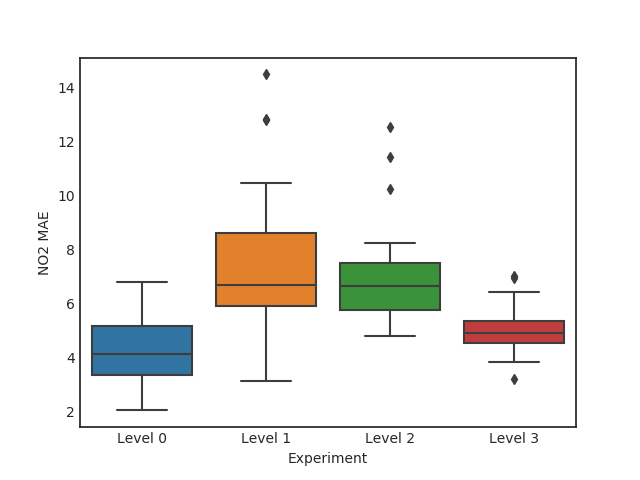
\includegraphics[width=\textwidth]{results/linear/no2.png}
\caption{NO2}
\end{subfigure}
\begin{subfigure}{0.45\textwidth}
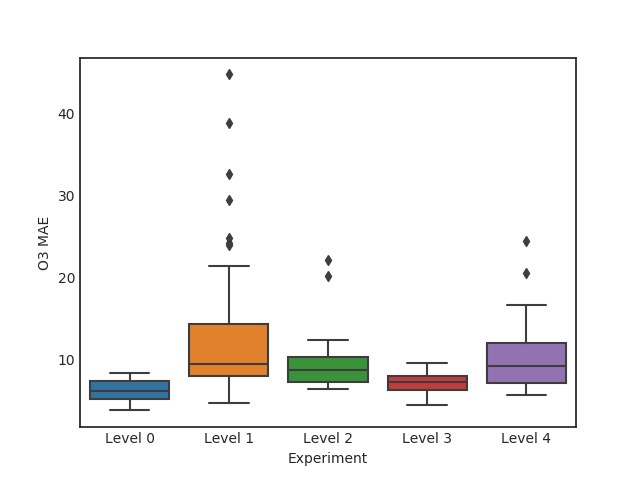
\includegraphics[width=\textwidth]{results/linear/o3.png}
\caption{O3}
\end{subfigure}
\caption{Results for linear regression. Error is in parts per billion}
\label{fig:results-linear}
\end{figure}

\begin{figure}[H]
\centering
\begin{subfigure}{0.45\textwidth}
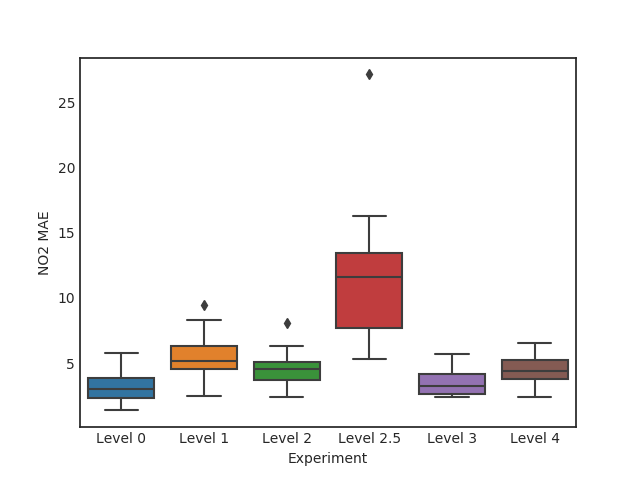
\includegraphics[width=\textwidth]{results/nn-2/no2.png}
\caption{NO2}
\end{subfigure}
\begin{subfigure}{0.45\textwidth}
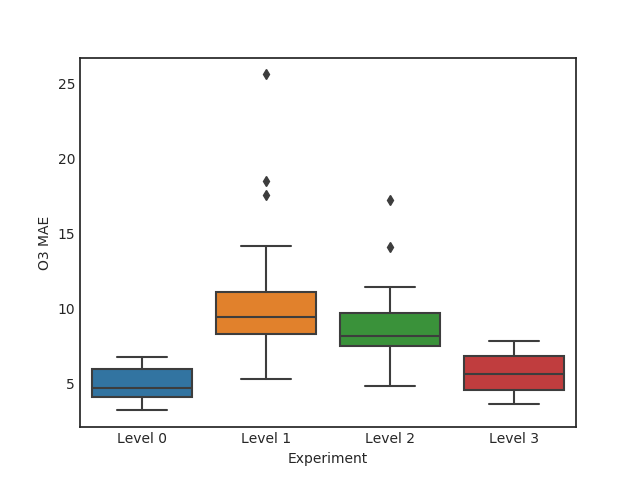
\includegraphics[width=\textwidth]{results/nn-2/o3.png}
\caption{O3}
\end{subfigure}
\caption{Results for NN[2]. Error is in parts per billion}
\label{fig:results-nn2}
\end{figure}

\begin{figure}[H]
\centering
\begin{subfigure}{0.45\textwidth}
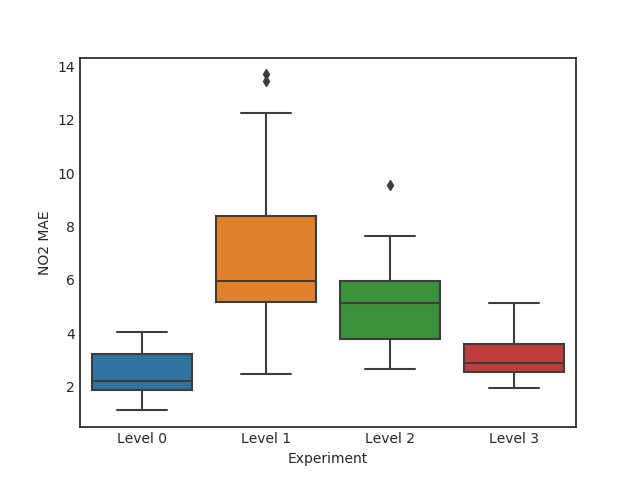
\includegraphics[width=\textwidth]{results/nn-4/no2.png}
\caption{NO2}
\end{subfigure}
\begin{subfigure}{0.45\textwidth}
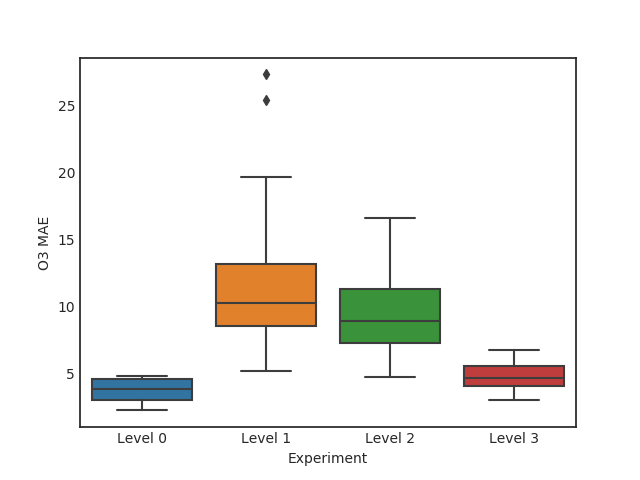
\includegraphics[width=\textwidth]{results/nn-4/o3.png}
\caption{O3}
\end{subfigure}
\caption{Results for NN[4]. Error is in parts per billion}
\label{fig:results-nn4}
\end{figure}

\begin{figure}[H]
\centering
\begin{subfigure}{0.45\textwidth}
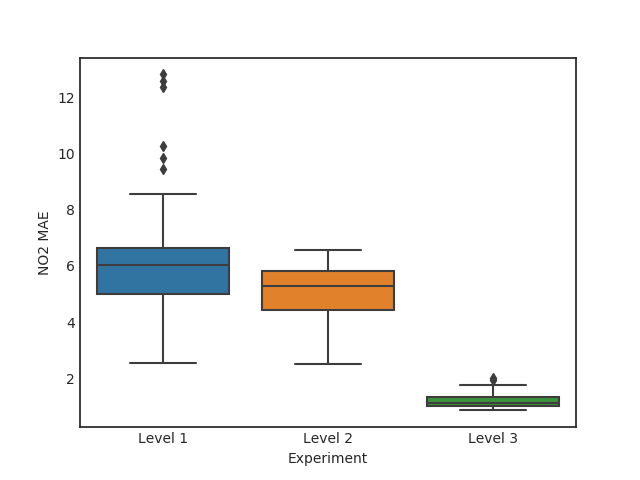
\includegraphics[width=\textwidth]{results/subu/no2.png}
\caption{NO2}
\end{subfigure}
\begin{subfigure}{0.45\textwidth}
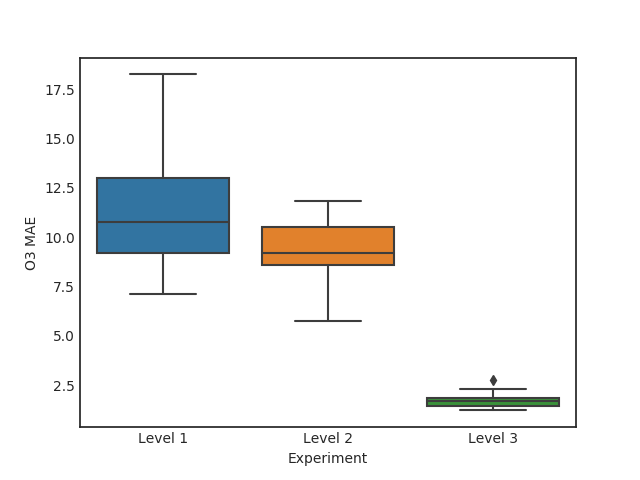
\includegraphics[width=\textwidth]{results/subu/o3.png}
\caption{O3}
\end{subfigure}
\caption{Results for Subu. Error is in parts per billion}
\label{fig:results-subu}
\end{figure}


We observe when comparing Level 1 error difference (Level 1 train minus Level 1 test), random forests suffer great
drops in performance.
This hints that RFs are overfitting to the training data, even if they
report the lowest test error for Level 0 and Level 3.  See \autoref{fig:generalization} for 
details.

\begin{figure}[H]
\centering
\begin{subfigure}{0.45\textwidth}
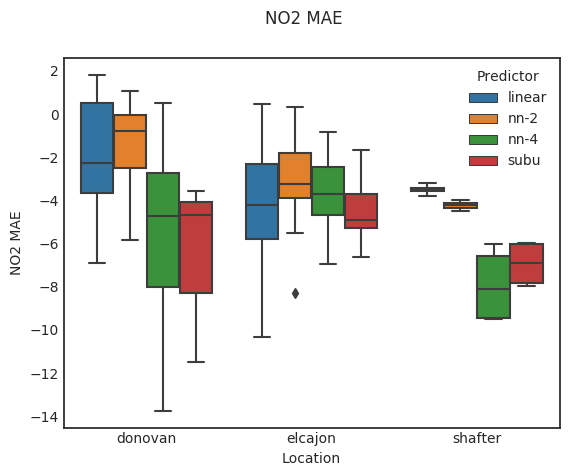
\includegraphics[width=\textwidth]{results/no2mae_diff.png}
\caption{NO2}
\end{subfigure}
\begin{subfigure}{0.45\textwidth}
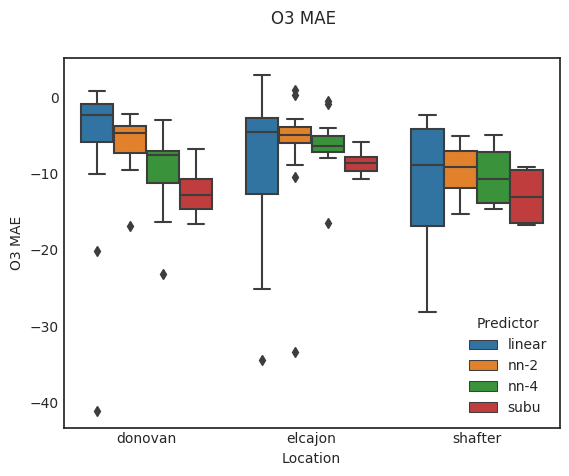
\includegraphics[width=\textwidth]{results/o3mae_diff.png}
\caption{O3}
\end{subfigure}
\caption{Level 1 difference plots. Train minus test errors for various models. A smaller value means that the models transfer better.}
\label{fig:generalization}
\end{figure}

\section{Neural representation learning}

We now present split-neural network results: we split
up calibration into two stages, a sensor model
and a pollutant model, which we will call $s_i$ and $c$
respectively.
Given a sensor readings $x$ from board $i$,
and environment readings $e$
we obtain a calibrated reading $y$ by simply passing it through
the sensor model, then the pollutant model, i.e.
\begin{align*}
    y = c(s_i(x), e)
\end{align*}
We can learn individual sensor models for each board,
but the pollutant model is shared across boards. This allows
us to pool data across boards to learn the pollutant model.
Furthermore, environment variables are only 
included in the pollutant model, which hopefully enables
a stronger fit with a very complex pollutant model.

Each $s_i(x)$ outputs a ``sensor representation'', which is chosen
to be some fixed dimension $d$. We hope that the sensor representation
contains the minimal information to produce calibrated readings.

We experiment with each $s_i$ being a linear regression model,
and $c$ being a deep neural network (two layers, 100 width ReLU). 
Each set of data we collect
is identified by a triplet of information (round, location, board number). In total, we have 25 of such datasets as defined in \autoref{tab:board-rotations}. To benchmark these split models, we train on all of these datasets, but
hold one triple out, resulting in a
total training set size of 24 datasets and test size of 1 dataset. This results in a total of 25 experiments
for which we boxplot the results.
We compare the split models to our four static models (Linear, NN[2], NN[4], Subu) by comparing the Split-NN performance on the held out dataset to the Level 2 performance of the four models.
Level 2 performance corresponds to training on two locations
and testing on the third. The split model has access to the same training data as the Level 2 models, but with the addition of data from other boards. The hope is this additional board data can help improve upon Level 2 performance, which can be thought of as the ``best'' possible transfer performance.

Notice that for some boards, we do not have the full three rounds of data (Boards 17 and 20). Therefore, there are no Level 2 results for these boards, but there are Level 1. For these two boards, in particular, we compare the split model to the Level 1 performance for a fair benchmark. This corresponds to the ``Training Size'' of 1.0 or 2.0 (Level 1 and Level 2).

\begin{figure}[H]
\begin{subfigure}{0.49\textwidth}
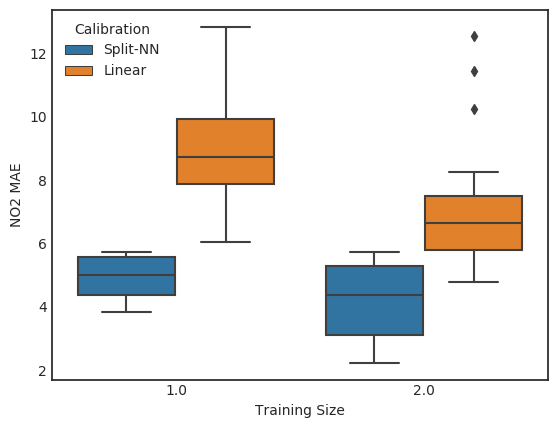
\includegraphics[width=\textwidth]{results/split/linear_relu2-100/linear/no2mae.png}
\caption{NO2 MAE}
\end{subfigure}
\begin{subfigure}{0.49\textwidth}
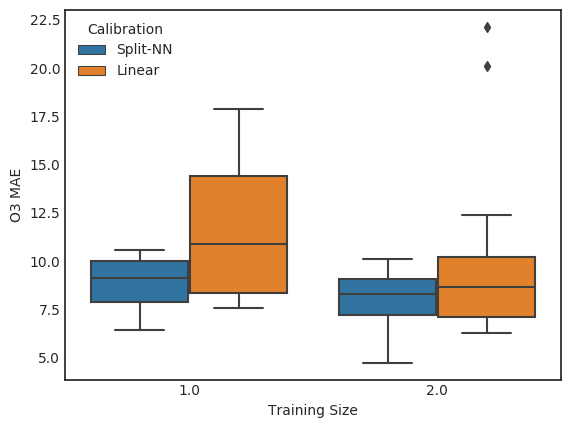
\includegraphics[width=\textwidth]{results/split/linear_relu2-100/linear/o3mae.png}
\caption{O3 MAE}
\end{subfigure}
\begin{subfigure}{0.49\textwidth}
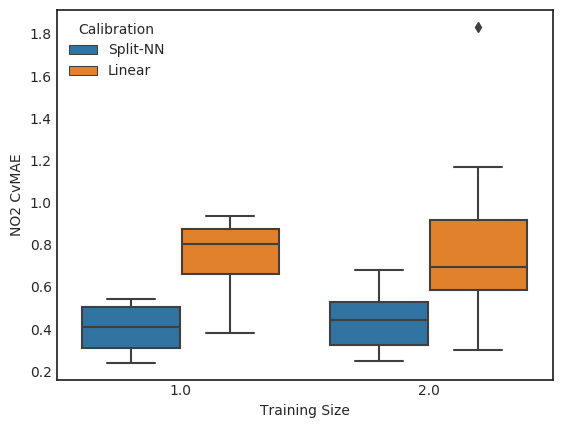
\includegraphics[width=\textwidth]{results/split/linear_relu2-100/linear/no2cvmae.png}
\caption{NO2 CvMAE}
\end{subfigure}
\begin{subfigure}{0.49\textwidth}
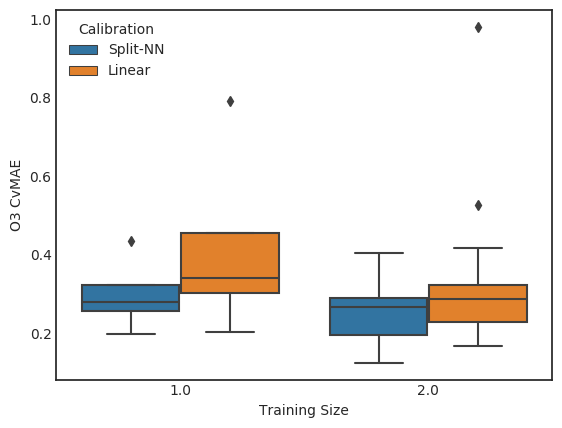
\includegraphics[width=\textwidth]{results/split/linear_relu2-100/linear/o3cvmae.png}
\caption{O3 CvMAE}
\end{subfigure}
\caption{Comparison of errors of Split NN and Linear. Training size corresponds to a Level 1 or Level 2 comparison.}
\end{figure}

\begin{figure}[H]
\begin{subfigure}{0.49\textwidth}
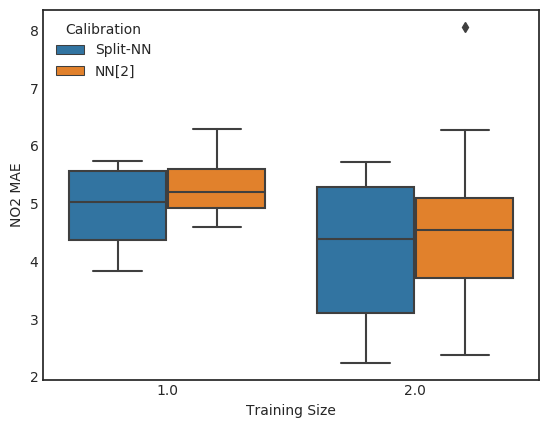
\includegraphics[width=\textwidth]{results/split/linear_relu2-100/nn-2/no2mae.png}
\caption{NO2 MAE}
\end{subfigure}
\begin{subfigure}{0.49\textwidth}
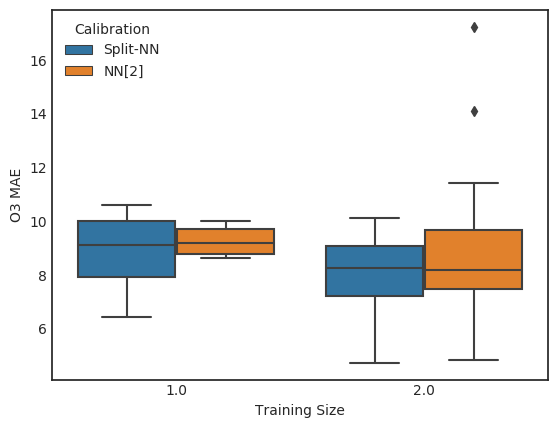
\includegraphics[width=\textwidth]{results/split/linear_relu2-100/nn-2/o3mae.png}
\caption{O3 MAE}
\end{subfigure}
\begin{subfigure}{0.49\textwidth}
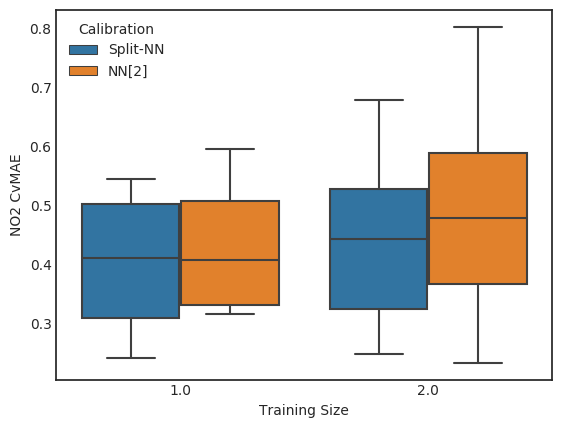
\includegraphics[width=\textwidth]{results/split/linear_relu2-100/nn-2/no2cvmae.png}
\caption{NO2 CvMAE}
\end{subfigure}
\begin{subfigure}{0.49\textwidth}
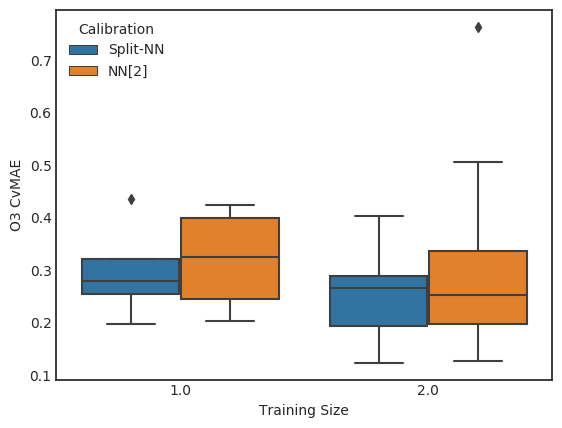
\includegraphics[width=\textwidth]{results/split/linear_relu2-100/nn-2/o3cvmae.png}
\caption{O3 CvMAE}
\end{subfigure}
\caption{Comparison of errors of Split NN and NN[2]. Training size corresponds to a Level 1 or Level 2 comparison.}
\end{figure}

\begin{figure}[H]
\begin{subfigure}{0.49\textwidth}
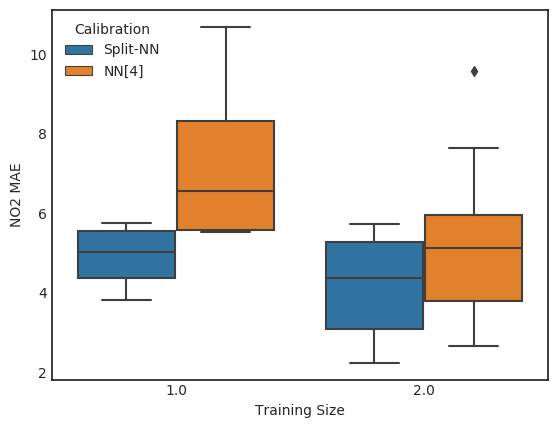
\includegraphics[width=\textwidth]{results/split/linear_relu2-100/nn-4/no2mae.png}
\caption{NO2 MAE}
\end{subfigure}
\begin{subfigure}{0.49\textwidth}
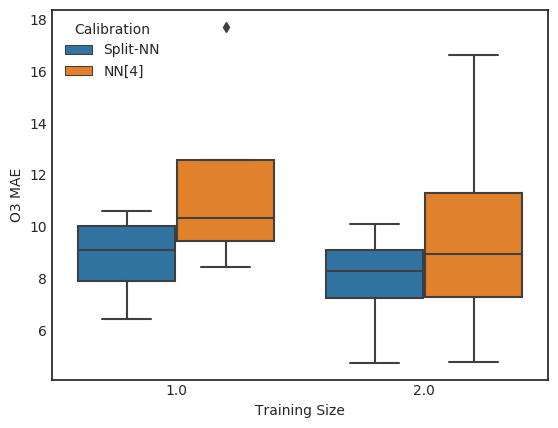
\includegraphics[width=\textwidth]{results/split/linear_relu2-100/nn-4/o3mae.png}
\caption{O3 MAE}
\end{subfigure}
\begin{subfigure}{0.49\textwidth}
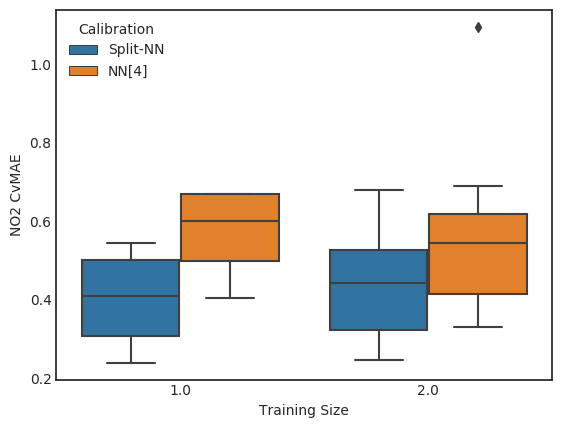
\includegraphics[width=\textwidth]{results/split/linear_relu2-100/nn-4/no2cvmae.png}
\caption{NO2 CvMAE}
\end{subfigure}
\begin{subfigure}{0.49\textwidth}
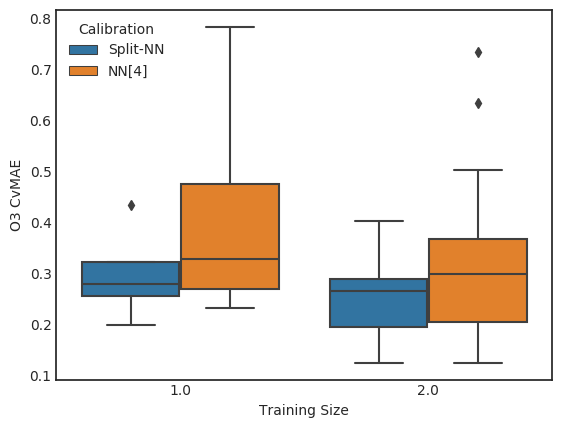
\includegraphics[width=\textwidth]{results/split/linear_relu2-100/nn-4/o3cvmae.png}
\caption{O3 CvMAE}
\end{subfigure}
\caption{Comparison of errors of Split NN and NN[4]. Training size corresponds to a Level 1 or Level 2 comparison.}
\end{figure}

\begin{figure}[H]
\begin{subfigure}{0.49\textwidth}
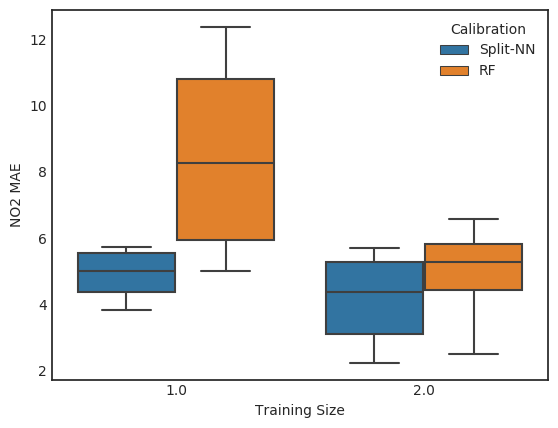
\includegraphics[width=\textwidth]{results/split/linear_relu2-100/subu/no2mae.png}
\caption{NO2 MAE}
\end{subfigure}
\begin{subfigure}{0.49\textwidth}
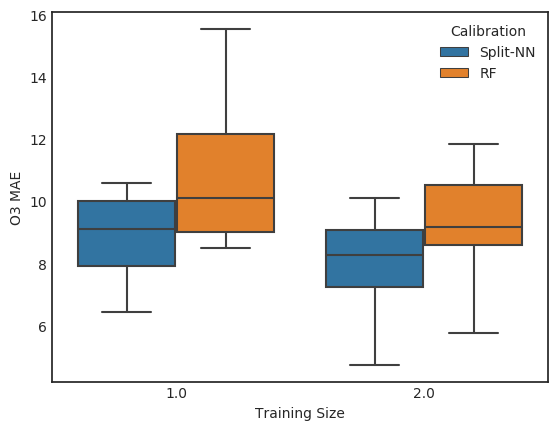
\includegraphics[width=\textwidth]{results/split/linear_relu2-100/subu/o3mae.png}
\caption{O3 MAE}
\end{subfigure}
\begin{subfigure}{0.49\textwidth}
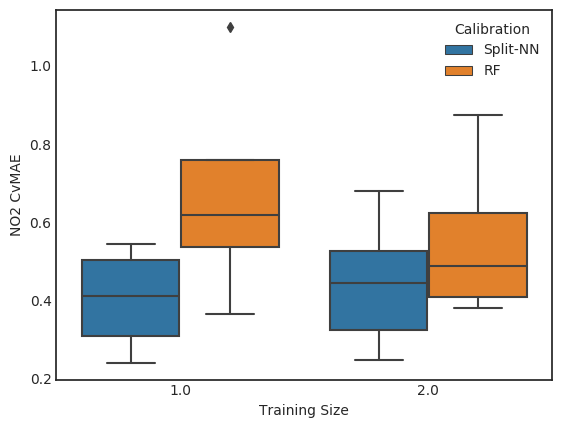
\includegraphics[width=\textwidth]{results/split/linear_relu2-100/subu/no2cvmae.png}
\caption{NO2 CvMAE}
\end{subfigure}
\begin{subfigure}{0.49\textwidth}
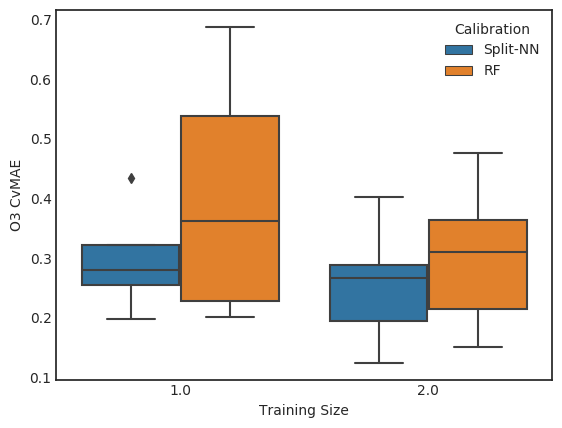
\includegraphics[width=\textwidth]{results/split/linear_relu2-100/subu/o3cvmae.png}
\caption{O3 CvMAE}
\end{subfigure}
\caption{Comparison of errors of Split NN and Subu. Training size corresponds to a Level 1 or Level 2 comparison.}
\end{figure}

To further accentuate the improvement, we can compare
the difference in performance between Split-NN and the four models. In these plots, a more negative value corresponds to a larger improvement.

\begin{figure}[H]
\begin{subfigure}{0.49\textwidth}
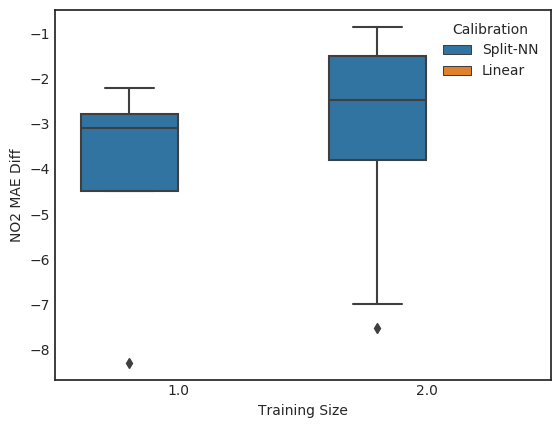
\includegraphics[width=\textwidth]{results/split/linear_relu2-100/linear/no2mae-diff.png}
\caption{NO2 MAE Difference}
\end{subfigure}
\begin{subfigure}{0.49\textwidth}
\includegraphics[width=\textwidth]{results/split/linear_relu2-100/linear/o3mae-diff.png}
\caption{O3 MAE Difference}
\end{subfigure}
\begin{subfigure}{0.49\textwidth}
\includegraphics[width=\textwidth]{results/split/linear_relu2-100/linear/no2cvmae-diff.png}
\caption{NO2 CvMAE Difference}
\end{subfigure}
\begin{subfigure}{0.49\textwidth}
\includegraphics[width=\textwidth]{results/split/linear_relu2-100/linear/o3cvmae-diff.png}
\caption{O3 CvMAE Difference}
\end{subfigure}
\caption{Comparison of errors of Split NN and Linear. Training size corresponds to a Level 1 or Level 2 comparison.}
\end{figure}

\begin{figure}[H]
\begin{subfigure}{0.49\textwidth}
\includegraphics[width=\textwidth]{results/split/linear_relu2-100/nn-2/no2mae-diff.png}
\caption{NO2 MAE Difference}
\end{subfigure}
\begin{subfigure}{0.49\textwidth}
\includegraphics[width=\textwidth]{results/split/linear_relu2-100/nn-2/o3mae-diff.png}
\caption{O3 MAE Difference}
\end{subfigure}
\begin{subfigure}{0.49\textwidth}
\includegraphics[width=\textwidth]{results/split/linear_relu2-100/nn-2/no2cvmae-diff.png}
\caption{NO2 CvMAE Difference}
\end{subfigure}
\begin{subfigure}{0.49\textwidth}
\includegraphics[width=\textwidth]{results/split/linear_relu2-100/nn-2/o3cvmae-diff.png}
\caption{O3 CvMAE Difference}
\end{subfigure}
\caption{Comparison of errors of Split NN and NN[2]. Training size corresponds to a Level 1 or Level 2 comparison.}
\end{figure}

\begin{figure}[H]
\begin{subfigure}{0.49\textwidth}
\includegraphics[width=\textwidth]{results/split/linear_relu2-100/nn-4/no2mae-diff.png}
\caption{NO2 MAE Difference}
\end{subfigure}
\begin{subfigure}{0.49\textwidth}
\includegraphics[width=\textwidth]{results/split/linear_relu2-100/nn-4/o3mae-diff.png}
\caption{O3 MAE Difference}
\end{subfigure}
\begin{subfigure}{0.49\textwidth}
\includegraphics[width=\textwidth]{results/split/linear_relu2-100/nn-4/no2cvmae-diff.png}
\caption{NO2 CvMAE Difference}
\end{subfigure}
\begin{subfigure}{0.49\textwidth}
\includegraphics[width=\textwidth]{results/split/linear_relu2-100/nn-4/o3cvmae-diff.png}
\caption{O3 CvMAE Difference}
\end{subfigure}
\caption{Comparison of errors of Split NN and NN[4]. Training size corresponds to a Level 1 or Level 2 comparison.}
\end{figure}

\begin{figure}[H]
\begin{subfigure}{0.49\textwidth}
\includegraphics[width=\textwidth]{results/split/linear_relu2-100/subu/no2mae-diff.png}
\caption{NO2 MAE Difference}
\end{subfigure}
\begin{subfigure}{0.49\textwidth}
\includegraphics[width=\textwidth]{results/split/linear_relu2-100/subu/o3mae-diff.png}
\caption{O3 MAE Difference}
\end{subfigure}
\begin{subfigure}{0.49\textwidth}
\includegraphics[width=\textwidth]{results/split/linear_relu2-100/subu/no2cvmae-diff.png}
\caption{NO2 CvMAE Difference}
\end{subfigure}
\begin{subfigure}{0.49\textwidth}
\includegraphics[width=\textwidth]{results/split/linear_relu2-100/subu/o3cvmae-diff.png}
\caption{O3 CvMAE Difference}
\end{subfigure}
\caption{Comparison of errors of Split NN and Subu. Training size corresponds to a Level 1 or Level 2 comparison.}
\end{figure}

\appendix
\setcounter{table}{0}
\renewcommand{\thetable}{\Alph{section}.\arabic{table}}

\section{Raw results for simple calibration models}
\label{sec:simpleresults}

\subsection{Benchmarks for linear regression}
\label{sec:results-lr}

\begin{table}[H]
\centering
\scriptsize
\begin{tabular}{lllrrrr}
\toprule
{} &             Model &  Testing Location &   NO2 MAE &    O3 MAE &  NO2 CvMAE &  O3 CvMAE \\
\midrule
11 &  (1, donovan, 19) &  (1, donovan, 19) &  2.817624 &  3.748897 &   0.669465 &  0.098983 \\
13 &  (1, donovan, 21) &  (1, donovan, 21) &  2.532854 &  4.071486 &   0.601804 &  0.107501 \\
10 &  (1, elcajon, 11) &  (1, elcajon, 11) &  2.042837 &  5.212672 &   0.380986 &  0.137718 \\
18 &  (1, elcajon, 12) &  (1, elcajon, 12) &  2.196888 &  5.192453 &   0.409716 &  0.137184 \\
5  &  (1, elcajon, 13) &  (1, elcajon, 13) &  2.087088 &  4.383210 &   0.389238 &  0.115804 \\
2  &  (1, shafter, 15) &  (1, shafter, 15) &  3.353189 &  5.572850 &   0.496553 &  0.169842 \\
6  &  (1, shafter, 18) &  (1, shafter, 18) &  2.309084 &  4.330305 &   0.413509 &  0.131661 \\
9  &  (2, donovan, 15) &  (2, donovan, 15) &  6.698192 &  7.547663 &   0.630592 &  0.175792 \\
12 &  (2, donovan, 18) &  (2, donovan, 18) &  6.324331 &  6.607726 &   0.609086 &  0.154963 \\
4  &  (2, donovan, 20) &  (2, donovan, 20) &  6.775750 &  7.562647 &   0.652561 &  0.177358 \\
3  &  (2, elcajon, 17) &  (2, elcajon, 17) &  3.379753 &  7.288420 &   0.300214 &  0.191092 \\
7  &  (2, elcajon, 19) &  (2, elcajon, 19) &  4.038051 &  7.618134 &   0.359570 &  0.199615 \\
14 &  (2, elcajon, 21) &  (2, elcajon, 21) &  3.970448 &  7.246587 &   0.353550 &  0.189880 \\
0  &  (3, donovan, 11) &  (3, donovan, 11) &  5.146091 &  5.509514 &   0.433960 &  0.184209 \\
1  &  (3, donovan, 12) &  (3, donovan, 12) &  3.858934 &  6.274502 &   0.325327 &  0.209866 \\
17 &  (3, donovan, 13) &  (3, donovan, 13) &  6.397274 &  8.225554 &   0.544893 &  0.276492 \\
8  &  (3, elcajon, 15) &  (3, elcajon, 15) &  3.956452 &  5.724768 &   0.249405 &  0.253835 \\
16 &  (3, elcajon, 18) &  (3, elcajon, 18) &  3.635693 &  4.002478 &   0.227972 &  0.177812 \\
15 &  (3, elcajon, 20) &  (3, elcajon, 20) &  4.175166 &  5.877268 &   0.261707 &  0.261232 \\
\bottomrule
\end{tabular}

\caption{Level 0 train results for linear regression}
\end{table}
\begin{table}[H]
\centering
\scriptsize
\begin{tabular}{lllrrrr}
\toprule
{} &             Model &  Testing Location &   NO2 MAE &    O3 MAE &  NO2 CvMAE &  O3 CvMAE \\
\midrule
16 &  (1, donovan, 19) &  (1, donovan, 19) &  2.850930 &  3.710558 &   0.673331 &  0.097286 \\
5  &  (1, donovan, 21) &  (1, donovan, 21) &  2.543194 &  4.096572 &   0.600650 &  0.107407 \\
8  &  (1, elcajon, 11) &  (1, elcajon, 11) &  2.053270 &  5.128018 &   0.378209 &  0.135625 \\
2  &  (1, elcajon, 12) &  (1, elcajon, 12) &  2.181817 &  5.183898 &   0.401887 &  0.137103 \\
9  &  (1, elcajon, 13) &  (1, elcajon, 13) &  2.072161 &  4.386177 &   0.381688 &  0.116005 \\
0  &  (1, shafter, 15) &  (1, shafter, 15) &  3.386877 &  5.589703 &   0.500763 &  0.171725 \\
6  &  (1, shafter, 18) &  (1, shafter, 18) &  2.313071 &  4.412545 &   0.419196 &  0.134887 \\
14 &  (2, donovan, 15) &  (2, donovan, 15) &  6.652718 &  7.528181 &   0.624712 &  0.175110 \\
22 &  (2, donovan, 18) &  (2, donovan, 18) &  6.385480 &  6.706138 &   0.605916 &  0.158235 \\
4  &  (2, donovan, 20) &  (2, donovan, 20) &  6.803972 &  7.533899 &   0.645627 &  0.177766 \\
13 &  (2, elcajon, 17) &  (2, elcajon, 17) &  3.350610 &  7.275296 &   0.297892 &  0.187986 \\
1  &  (2, elcajon, 19) &  (2, elcajon, 19) &  4.136211 &  7.747041 &   0.363729 &  0.200693 \\
3  &  (2, elcajon, 21) &  (2, elcajon, 21) &  4.037583 &  7.344045 &   0.355056 &  0.190253 \\
20 &  (2, shafter, 11) &  (2, shafter, 11) &  4.416675 &  7.262233 &   0.325816 &  0.230545 \\
21 &  (2, shafter, 12) &  (2, shafter, 12) &  4.619718 &  6.987870 &   0.344165 &  0.221812 \\
11 &  (2, shafter, 13) &  (2, shafter, 13) &  4.576023 &  7.411089 &   0.339026 &  0.233867 \\
23 &  (3, donovan, 11) &  (3, donovan, 11) &  5.193754 &  5.600240 &   0.431705 &  0.188033 \\
15 &  (3, donovan, 12) &  (3, donovan, 12) &  3.967916 &  6.324312 &   0.330162 &  0.212043 \\
12 &  (3, donovan, 13) &  (3, donovan, 13) &  6.487443 &  8.338580 &   0.544654 &  0.280263 \\
24 &  (3, elcajon, 15) &  (3, elcajon, 15) &  3.975396 &  5.762910 &   0.249059 &  0.256456 \\
17 &  (3, elcajon, 18) &  (3, elcajon, 18) &  3.618518 &  4.013838 &   0.226705 &  0.178048 \\
10 &  (3, elcajon, 20) &  (3, elcajon, 20) &  4.169921 &  5.865262 &   0.261620 &  0.259674 \\
18 &  (3, shafter, 17) &  (3, shafter, 17) &  5.385507 &  6.088492 &   0.393443 &  0.269503 \\
7  &  (3, shafter, 19) &  (3, shafter, 19) &  5.993148 &  6.998718 &   0.437834 &  0.309794 \\
19 &  (3, shafter, 21) &  (3, shafter, 21) &  4.812474 &  5.096993 &   0.351579 &  0.225615 \\
\bottomrule
\end{tabular}

\caption{Level 0 test results for linear regression}
\end{table}

\begin{table}[H]
\centering
\scriptsize
\begin{tabular}{lllrrrr}
\toprule
{} &             Model & Testing Location &   NO2 MAE &    O3 MAE &  NO2 CvMAE &  O3 CvMAE \\
\midrule
20 &  (1, donovan, 19) &     (2, elcajon) &  2.850930 &  3.710558 &   0.673331 &  0.097286 \\
21 &  (1, donovan, 19) &     (3, shafter) &  2.850930 &  3.710558 &   0.673331 &  0.097286 \\
24 &  (1, donovan, 21) &     (2, elcajon) &  2.543194 &  4.096572 &   0.600650 &  0.107407 \\
25 &  (1, donovan, 21) &     (3, shafter) &  2.543194 &  4.096572 &   0.600650 &  0.107407 \\
18 &  (1, elcajon, 11) &     (2, shafter) &  2.053270 &  5.128018 &   0.378209 &  0.135625 \\
19 &  (1, elcajon, 11) &     (3, donovan) &  2.053270 &  5.128018 &   0.378209 &  0.135625 \\
33 &  (1, elcajon, 12) &     (2, shafter) &  2.181817 &  5.183898 &   0.401887 &  0.137103 \\
34 &  (1, elcajon, 12) &     (3, donovan) &  2.181817 &  5.183898 &   0.401887 &  0.137103 \\
8  &  (1, elcajon, 13) &     (2, shafter) &  2.072161 &  4.386177 &   0.381688 &  0.116005 \\
9  &  (1, elcajon, 13) &     (3, donovan) &  2.072161 &  4.386177 &   0.381688 &  0.116005 \\
4  &  (1, shafter, 15) &     (2, donovan) &  3.386877 &  5.589703 &   0.500763 &  0.171725 \\
5  &  (1, shafter, 15) &     (3, elcajon) &  3.386877 &  5.589703 &   0.500763 &  0.171725 \\
10 &  (1, shafter, 18) &     (2, donovan) &  2.313071 &  4.412545 &   0.419196 &  0.134887 \\
11 &  (1, shafter, 18) &     (3, elcajon) &  2.313071 &  4.412545 &   0.419196 &  0.134887 \\
16 &  (2, donovan, 15) &     (1, shafter) &  6.652718 &  7.528181 &   0.624712 &  0.175110 \\
17 &  (2, donovan, 15) &     (3, elcajon) &  6.652718 &  7.528181 &   0.624712 &  0.175110 \\
22 &  (2, donovan, 18) &     (1, shafter) &  6.385480 &  6.706138 &   0.605916 &  0.158235 \\
23 &  (2, donovan, 18) &     (3, elcajon) &  6.385480 &  6.706138 &   0.605916 &  0.158235 \\
7  &  (2, donovan, 20) &     (3, elcajon) &  6.803972 &  7.533899 &   0.645627 &  0.177766 \\
6  &  (2, elcajon, 17) &     (3, shafter) &  3.350610 &  7.275296 &   0.297892 &  0.187986 \\
12 &  (2, elcajon, 19) &     (1, donovan) &  4.136211 &  7.747041 &   0.363729 &  0.200693 \\
13 &  (2, elcajon, 19) &     (3, shafter) &  4.136211 &  7.747041 &   0.363729 &  0.200693 \\
26 &  (2, elcajon, 21) &     (1, donovan) &  4.037583 &  7.344045 &   0.355056 &  0.190253 \\
27 &  (2, elcajon, 21) &     (3, shafter) &  4.037583 &  7.344045 &   0.355056 &  0.190253 \\
0  &  (3, donovan, 11) &     (1, elcajon) &  5.193754 &  5.600240 &   0.431705 &  0.188033 \\
1  &  (3, donovan, 11) &     (2, shafter) &  5.193754 &  5.600240 &   0.431705 &  0.188033 \\
2  &  (3, donovan, 12) &     (1, elcajon) &  3.967916 &  6.324312 &   0.330162 &  0.212043 \\
3  &  (3, donovan, 12) &     (2, shafter) &  3.967916 &  6.324312 &   0.330162 &  0.212043 \\
31 &  (3, donovan, 13) &     (1, elcajon) &  6.487443 &  8.338580 &   0.544654 &  0.280263 \\
32 &  (3, donovan, 13) &     (2, shafter) &  6.487443 &  8.338580 &   0.544654 &  0.280263 \\
14 &  (3, elcajon, 15) &     (1, shafter) &  3.975396 &  5.762910 &   0.249059 &  0.256456 \\
15 &  (3, elcajon, 15) &     (2, donovan) &  3.975396 &  5.762910 &   0.249059 &  0.256456 \\
29 &  (3, elcajon, 18) &     (1, shafter) &  3.618518 &  4.013838 &   0.226705 &  0.178048 \\
30 &  (3, elcajon, 18) &     (2, donovan) &  3.618518 &  4.013838 &   0.226705 &  0.178048 \\
28 &  (3, elcajon, 20) &     (2, donovan) &  4.169921 &  5.865262 &   0.261620 &  0.259674 \\
\bottomrule
\end{tabular}

\caption{Level 1 train results for linear regression}
\end{table}
\begin{table}[H]
\centering
\scriptsize
\begin{tabular}{lllrrrr}
\toprule
{} &             Model & Testing Location &    NO2 MAE &     O3 MAE &  NO2 CvMAE &  O3 CvMAE \\
\midrule
29 &  (1, donovan, 19) &     (2, elcajon) &   4.721054 &  13.743547 &   0.415159 &  0.356037 \\
30 &  (1, donovan, 19) &     (3, shafter) &   9.750380 &  44.837383 &   0.712322 &  1.984698 \\
9  &  (1, donovan, 21) &     (2, elcajon) &   5.435679 &  11.265806 &   0.478001 &  0.291849 \\
10 &  (1, donovan, 21) &     (3, shafter) &   8.163074 &  24.216401 &   0.596360 &  1.071923 \\
15 &  (1, elcajon, 11) &     (2, shafter) &   5.859866 &  23.973826 &   0.432280 &  0.761068 \\
16 &  (1, elcajon, 11) &     (3, donovan) &   6.238380 &  11.191060 &   0.518534 &  0.375750 \\
4  &  (1, elcajon, 12) &     (2, shafter) &   6.504934 &  17.526472 &   0.484612 &  0.556333 \\
5  &  (1, elcajon, 12) &     (3, donovan) &   6.446498 &  10.332413 &   0.536399 &  0.346427 \\
17 &  (1, elcajon, 13) &     (2, shafter) &   6.987382 &  29.507606 &   0.517678 &  0.931151 \\
18 &  (1, elcajon, 13) &     (3, donovan) &  10.459595 &  38.840301 &   0.878137 &  1.305440 \\
0  &  (1, shafter, 15) &     (2, donovan) &   6.879212 &  18.603261 &   0.645980 &  0.432722 \\
1  &  (1, shafter, 15) &     (3, elcajon) &   6.870887 &   7.834289 &   0.430462 &  0.348635 \\
11 &  (1, shafter, 18) &     (2, donovan) &   6.108138 &  32.634696 &   0.579599 &  0.770032 \\
12 &  (1, shafter, 18) &     (3, elcajon) &   5.490944 &   9.172539 &   0.344015 &  0.406881 \\
25 &  (2, donovan, 15) &     (1, shafter) &   9.377802 &   8.475076 &   1.386546 &  0.260368 \\
26 &  (2, donovan, 15) &     (3, elcajon) &   6.425870 &   7.199287 &   0.402582 &  0.320377 \\
40 &  (2, donovan, 18) &     (1, shafter) &   8.651816 &   8.316647 &   1.567962 &  0.254231 \\
41 &  (2, donovan, 18) &     (3, elcajon) &   6.229479 &   5.859996 &   0.390285 &  0.259941 \\
8  &  (2, donovan, 20) &     (3, elcajon) &   6.052090 &   7.586682 &   0.379707 &  0.335886 \\
24 &  (2, elcajon, 17) &     (3, shafter) &  12.827964 &  17.886811 &   0.937158 &  0.791748 \\
2  &  (2, elcajon, 19) &     (1, donovan) &   4.800626 &   4.762190 &   1.133809 &  0.124859 \\
3  &  (2, elcajon, 19) &     (3, shafter) &  14.483825 &  21.333860 &   1.058128 &  0.944329 \\
6  &  (2, elcajon, 21) &     (1, donovan) &   3.583996 &   4.596593 &   0.846466 &  0.120517 \\
7  &  (2, elcajon, 21) &     (3, shafter) &  12.789354 &   9.587360 &   0.934337 &  0.424378 \\
36 &  (2, shafter, 11) &     (1, elcajon) &   7.210789 &   7.536208 &   1.328214 &  0.199317 \\
37 &  (2, shafter, 11) &     (3, donovan) &   6.656738 &   9.714873 &   0.553308 &  0.326186 \\
38 &  (2, shafter, 12) &     (1, elcajon) &   6.664027 &   7.139145 &   1.227502 &  0.188815 \\
39 &  (2, shafter, 12) &     (3, donovan) &   6.732293 &   9.466997 &   0.560180 &  0.317411 \\
20 &  (2, shafter, 13) &     (1, elcajon) &   9.198244 &   9.330914 &   1.694300 &  0.246783 \\
21 &  (2, shafter, 13) &     (3, donovan) &   9.655395 &  14.511711 &   0.810620 &  0.487745 \\
42 &  (3, donovan, 11) &     (1, elcajon) &   3.692888 &   7.873262 &   0.680223 &  0.208231 \\
43 &  (3, donovan, 11) &     (2, shafter) &   9.106516 &   7.761055 &   0.671783 &  0.246381 \\
27 &  (3, donovan, 12) &     (1, elcajon) &   7.332869 &   8.791024 &   1.350701 &  0.232504 \\
28 &  (3, donovan, 12) &     (2, shafter) &   9.222817 &   9.973596 &   0.687092 &  0.316586 \\
22 &  (3, donovan, 13) &     (1, elcajon) &   4.669914 &   8.973694 &   0.860190 &  0.237335 \\
23 &  (3, donovan, 13) &     (2, shafter) &   5.636151 &  12.978008 &   0.417569 &  0.409538 \\
44 &  (3, elcajon, 15) &     (1, shafter) &   4.827194 &   8.805387 &   0.713720 &  0.270516 \\
45 &  (3, elcajon, 15) &     (2, donovan) &   6.621335 &   8.375271 &   0.621765 &  0.194813 \\
31 &  (3, elcajon, 18) &     (1, shafter) &   4.991286 &   6.798044 &   0.904567 &  0.207809 \\
32 &  (3, elcajon, 18) &     (2, donovan) &   7.125273 &   7.871634 &   0.676115 &  0.185735 \\
19 &  (3, elcajon, 20) &     (2, donovan) &   8.969028 &   8.574747 &   0.851068 &  0.202325 \\
33 &  (3, shafter, 17) &     (2, elcajon) &   8.463228 &  13.245548 &   0.752440 &  0.342250 \\
13 &  (3, shafter, 19) &     (1, donovan) &   7.840513 &  24.786326 &   1.851768 &  0.649866 \\
14 &  (3, shafter, 19) &     (2, elcajon) &   6.344760 &  10.436176 &   0.557944 &  0.270357 \\
34 &  (3, shafter, 21) &     (1, donovan) &   3.141038 &   8.195038 &   0.741848 &  0.214863 \\
35 &  (3, shafter, 21) &     (2, elcajon) &   8.051262 &   8.951980 &   0.708009 &  0.231908 \\
\bottomrule
\end{tabular}

\caption{Level 1 test results for linear regression}
\end{table}

\begin{table}[H]
\centering
\scriptsize
\begin{tabular}{lrrrrr}
\toprule
{} &  Model &   NO2 MAE &    O3 MAE &  NO2 CvMAE &  O3 CvMAE \\
\midrule
0 &   15.0 &  4.641259 &  6.699894 &   0.333736 &  0.265419 \\
1 &   15.0 &  4.929196 &  6.500251 &   0.340439 &  0.232236 \\
2 &   18.0 &  4.018519 &  4.634545 &   0.264144 &  0.196838 \\
3 &   15.0 &  6.333364 &  8.627098 &   0.668106 &  0.226853 \\
4 &   18.0 &  4.522039 &  5.091525 &   0.312840 &  0.182231 \\
5 &   18.0 &  6.495421 &  7.563168 &   0.657163 &  0.185959 \\
\bottomrule
\end{tabular}

\caption{Level 2 train results for linear regression}
\end{table}
\begin{table}[H]
\centering
\scriptsize
\begin{tabular}{lrrrrr}
\toprule
{} &  Model &   NO2 MAE &     O3 MAE &  NO2 CvMAE &  O3 CvMAE \\
\midrule
0 &   15.0 &  6.869842 &  11.226675 &   0.646421 &  0.261411 \\
1 &   15.0 &  7.321198 &  11.003615 &   0.883139 &  0.334109 \\
2 &   18.0 &  6.870132 &   7.879366 &   0.659678 &  0.185011 \\
3 &   15.0 &  5.372633 &   7.022111 &   0.338260 &  0.311585 \\
4 &   18.0 &  7.172693 &  10.826301 &   0.902242 &  0.321467 \\
5 &   18.0 &  4.804197 &   5.440729 &   0.301191 &  0.241634 \\
\bottomrule
\end{tabular}

\caption{Level 2 test results for linear regression}
\end{table}

\begin{table}[H]
\centering
\scriptsize
\begin{tabular}{lrrrrr}
\toprule
{} &  Model &   NO2 MAE &    O3 MAE &  NO2 CvMAE &  O3 CvMAE \\
\midrule
0 &   20.0 &  4.887944 &  6.444643 &   0.338554 &  0.230672 \\
1 &   21.0 &  3.676891 &  6.226018 &   0.426252 &  0.163153 \\
2 &   18.0 &  4.786327 &  5.496566 &   0.341934 &  0.193514 \\
3 &   19.0 &  3.806506 &  6.421858 &   0.441278 &  0.168285 \\
4 &   15.0 &  5.301882 &  7.213557 &   0.401219 &  0.248596 \\
5 &   17.0 &  3.379753 &  7.288420 &   0.300214 &  0.191092 \\
6 &   11.0 &  4.578849 &  5.799257 &   0.432929 &  0.184273 \\
7 &   12.0 &  4.144483 &  6.673056 &   0.391018 &  0.212085 \\
8 &   13.0 &  5.568965 &  7.949884 &   0.535982 &  0.252475 \\
\bottomrule
\end{tabular}

\caption{Level 3 train results for linear regression}
\end{table}
\begin{table}[H]
\centering
\scriptsize
\begin{tabular}{lllrrrr}
\toprule
{} & Model &          Test &   NO2 MAE &    O3 MAE &  NO2 CvMAE &  O3 CvMAE \\
\midrule
0  &    11 &  (1, elcajon) &  4.786708 &  6.411199 &   0.881703 &  0.169563 \\
1  &    11 &  (3, donovan) &  5.559995 &  6.068253 &   0.462147 &  0.203747 \\
2  &    11 &  (2, shafter) &  4.910759 &  7.574027 &   0.362264 &  0.240443 \\
3  &    17 &  (3, shafter) &  5.377550 &  6.764763 &   0.392861 &  0.299438 \\
4  &    17 &  (2, elcajon) &  4.537174 &  8.539158 &   0.403386 &  0.220642 \\
5  &    18 &  (1, shafter) &  4.547233 &  6.491199 &   0.824092 &  0.198429 \\
6  &    18 &  (2, donovan) &  6.439269 &  7.183452 &   0.611020 &  0.169497 \\
7  &    18 &  (3, elcajon) &  3.826094 &  4.370092 &   0.239710 &  0.193851 \\
8  &    13 &  (1, elcajon) &  4.537953 &  6.181242 &   0.835883 &  0.163481 \\
9  &    13 &  (3, donovan) &  7.022886 &  9.302385 &   0.589607 &  0.312657 \\
10 &    13 &  (2, shafter) &  4.708530 &  8.672204 &   0.348844 &  0.273663 \\
11 &    12 &  (1, elcajon) &  4.896463 &  6.899156 &   0.901920 &  0.182468 \\
12 &    12 &  (3, donovan) &  5.034365 &  7.162217 &   0.418899 &  0.240136 \\
13 &    12 &  (2, shafter) &  5.025221 &  8.150344 &   0.374375 &  0.258712 \\
14 &    20 &  (2, donovan) &  6.956268 &  7.573315 &   0.660078 &  0.178696 \\
15 &    20 &  (3, elcajon) &  4.540978 &  6.151124 &   0.284900 &  0.272330 \\
16 &    15 &  (1, shafter) &  4.222153 &  7.308019 &   0.624262 &  0.224514 \\
17 &    15 &  (2, donovan) &  6.364974 &  7.939930 &   0.597692 &  0.184687 \\
18 &    15 &  (3, elcajon) &  4.369725 &  6.194737 &   0.273764 &  0.275673 \\
19 &    19 &  (3, shafter) &  6.290076 &  7.964287 &   0.459527 &  0.352534 \\
20 &    19 &  (1, donovan) &  4.316830 &  9.360724 &   1.019546 &  0.245426 \\
21 &    19 &  (2, elcajon) &  5.207876 &  9.523878 &   0.457968 &  0.246723 \\
22 &    21 &  (3, shafter) &  5.370388 &  5.512022 &   0.392338 &  0.243986 \\
23 &    21 &  (1, donovan) &  3.215714 &  5.063684 &   0.759485 &  0.132763 \\
24 &    21 &  (2, elcajon) &  5.113928 &  7.945304 &   0.449707 &  0.205829 \\
\bottomrule
\end{tabular}

\caption{Level 3 test results for linear regression}
\end{table}

\subsection{Benchmarks for NN[2]}
\label{sec:results-nn2}

\begin{table}[H]
\centering
\scriptsize
\begin{tabular}{lllrrrr}
\toprule
{} &             Model &  Testing Location &   NO2 MAE &    O3 MAE &  NO2 CvMAE &  O3 CvMAE \\
\midrule
16 &  (1, donovan, 19) &  (1, donovan, 19) &  2.376601 &  4.059605 &   0.564678 &  0.107187 \\
5  &  (1, donovan, 21) &  (1, donovan, 21) &  2.106573 &  3.643729 &   0.500520 &  0.096207 \\
8  &  (1, elcajon, 11) &  (1, elcajon, 11) &  1.363333 &  4.308309 &   0.254259 &  0.113825 \\
2  &  (1, elcajon, 12) &  (1, elcajon, 12) &  1.731689 &  3.433356 &   0.322957 &  0.090709 \\
9  &  (1, elcajon, 13) &  (1, elcajon, 13) &  1.592846 &  3.237433 &   0.297063 &  0.085532 \\
0  &  (1, shafter, 15) &  (1, shafter, 15) &  2.197847 &  3.945468 &   0.325466 &  0.120245 \\
6  &  (1, shafter, 18) &  (1, shafter, 18) &  2.200961 &  4.377567 &   0.394146 &  0.133098 \\
14 &  (2, donovan, 15) &  (2, donovan, 15) &  5.774000 &  6.602082 &   0.543585 &  0.153768 \\
22 &  (2, donovan, 18) &  (2, donovan, 18) &  5.147102 &  6.150489 &   0.495709 &  0.144240 \\
4  &  (2, donovan, 20) &  (2, donovan, 20) &  5.239533 &  6.653606 &   0.504610 &  0.156039 \\
13 &  (2, elcajon, 17) &  (2, elcajon, 17) &  2.531008 &  5.177073 &   0.224822 &  0.135736 \\
1  &  (2, elcajon, 19) &  (2, elcajon, 19) &  3.021720 &  6.658900 &   0.269070 &  0.174481 \\
3  &  (2, elcajon, 21) &  (2, elcajon, 21) &  2.697276 &  5.373738 &   0.240180 &  0.140806 \\
20 &  (2, shafter, 11) &  (2, shafter, 11) &  3.871853 &  5.892196 &   0.288404 &  0.186746 \\
21 &  (2, shafter, 12) &  (2, shafter, 12) &  4.011850 &  6.202820 &   0.298460 &  0.196155 \\
11 &  (2, shafter, 13) &  (2, shafter, 13) &  3.847771 &  6.404214 &   0.283740 &  0.203909 \\
23 &  (3, donovan, 11) &  (3, donovan, 11) &  3.364954 &  4.612540 &   0.283760 &  0.154219 \\
15 &  (3, donovan, 12) &  (3, donovan, 12) &  3.123734 &  4.774751 &   0.263346 &  0.159704 \\
12 &  (3, donovan, 13) &  (3, donovan, 13) &  3.544877 &  5.484555 &   0.301938 &  0.184356 \\
24 &  (3, elcajon, 15) &  (3, elcajon, 15) &  2.328371 &  4.167490 &   0.146775 &  0.184786 \\
17 &  (3, elcajon, 18) &  (3, elcajon, 18) &  2.520757 &  3.234963 &   0.158061 &  0.143715 \\
10 &  (3, elcajon, 20) &  (3, elcajon, 20) &  2.357596 &  3.846291 &   0.147778 &  0.170959 \\
18 &  (3, shafter, 17) &  (3, shafter, 17) &  3.481401 &  4.433496 &   0.254340 &  0.194426 \\
7  &  (3, shafter, 19) &  (3, shafter, 19) &  3.921369 &  4.727419 &   0.286482 &  0.207316 \\
19 &  (3, shafter, 21) &  (3, shafter, 21) &  3.053778 &  4.597083 &   0.223099 &  0.201600 \\
\bottomrule
\end{tabular}

\caption{Level 0 train results for NN[2]}
\end{table}
\begin{table}[H]
\centering
\scriptsize
\begin{tabular}{lllrrrr}
\toprule
{} &             Model &  Testing Location &   NO2 MAE &    O3 MAE &  NO2 CvMAE &  O3 CvMAE \\
\midrule
16 &  (1, donovan, 19) &  (1, donovan, 19) &  2.406302 &  4.068393 &   0.568319 &  0.106668 \\
5  &  (1, donovan, 21) &  (1, donovan, 21) &  2.121591 &  3.700573 &   0.501076 &  0.097024 \\
8  &  (1, elcajon, 11) &  (1, elcajon, 11) &  1.372707 &  4.321155 &   0.252850 &  0.114286 \\
2  &  (1, elcajon, 12) &  (1, elcajon, 12) &  1.751919 &  3.411224 &   0.322700 &  0.090220 \\
9  &  (1, elcajon, 13) &  (1, elcajon, 13) &  1.587393 &  3.206342 &   0.292395 &  0.084801 \\
0  &  (1, shafter, 15) &  (1, shafter, 15) &  2.201070 &  3.989497 &   0.325437 &  0.122564 \\
6  &  (1, shafter, 18) &  (1, shafter, 18) &  2.302697 &  4.502786 &   0.417316 &  0.137645 \\
14 &  (2, donovan, 15) &  (2, donovan, 15) &  5.782659 &  6.622596 &   0.543010 &  0.154045 \\
22 &  (2, donovan, 18) &  (2, donovan, 18) &  5.275075 &  6.264368 &   0.500550 &  0.147811 \\
4  &  (2, donovan, 20) &  (2, donovan, 20) &  5.336130 &  6.772800 &   0.506344 &  0.159808 \\
13 &  (2, elcajon, 17) &  (2, elcajon, 17) &  2.556621 &  5.126892 &   0.227301 &  0.132473 \\
1  &  (2, elcajon, 19) &  (2, elcajon, 19) &  3.082288 &  6.774753 &   0.271049 &  0.175505 \\
3  &  (2, elcajon, 21) &  (2, elcajon, 21) &  2.762940 &  5.463632 &   0.242967 &  0.141540 \\
20 &  (2, shafter, 11) &  (2, shafter, 11) &  3.874197 &  5.946993 &   0.285798 &  0.188792 \\
21 &  (2, shafter, 12) &  (2, shafter, 12) &  4.048163 &  6.254481 &   0.301585 &  0.198533 \\
11 &  (2, shafter, 13) &  (2, shafter, 13) &  3.882250 &  6.439484 &   0.287627 &  0.203206 \\
23 &  (3, donovan, 11) &  (3, donovan, 11) &  3.447279 &  4.675427 &   0.286538 &  0.156982 \\
15 &  (3, donovan, 12) &  (3, donovan, 12) &  3.205964 &  4.806858 &   0.266761 &  0.161165 \\
12 &  (3, donovan, 13) &  (3, donovan, 13) &  3.665248 &  5.595738 &   0.307716 &  0.188075 \\
24 &  (3, elcajon, 15) &  (3, elcajon, 15) &  2.317087 &  4.174768 &   0.145166 &  0.185782 \\
17 &  (3, elcajon, 18) &  (3, elcajon, 18) &  2.540051 &  3.222305 &   0.159138 &  0.142937 \\
10 &  (3, elcajon, 20) &  (3, elcajon, 20) &  2.365656 &  3.836465 &   0.148421 &  0.169852 \\
18 &  (3, shafter, 17) &  (3, shafter, 17) &  3.498404 &  4.454751 &   0.255579 &  0.197187 \\
7  &  (3, shafter, 19) &  (3, shafter, 19) &  3.902972 &  4.688188 &   0.285135 &  0.207520 \\
19 &  (3, shafter, 21) &  (3, shafter, 21) &  3.050720 &  4.577955 &   0.222873 &  0.202640 \\
\bottomrule
\end{tabular}

\caption{Level 0 test results for NN[2]}
\end{table}

\begin{table}[H]
\centering
\scriptsize
\begin{tabular}{llrrrr}
\toprule
{} &             Model &   NO2 MAE &    O3 MAE &  NO2 CvMAE &  O3 CvMAE \\
\midrule
0  &  (3, donovan, 11) &  3.447082 &  4.786970 &   0.289843 &  0.160186 \\
1  &  (3, donovan, 12) &  3.108793 &  4.917466 &   0.261397 &  0.164556 \\
2  &  (1, shafter, 15) &  4.740303 &  6.973310 &   0.571812 &  0.211735 \\
3  &  (2, donovan, 20) &  5.470669 &  6.771672 &   0.525300 &  0.159001 \\
4  &  (1, elcajon, 13) &  1.563195 &  3.343776 &   0.290807 &  0.088361 \\
5  &  (1, shafter, 18) &  5.726096 &  8.088070 &   0.720277 &  0.240160 \\
6  &  (2, elcajon, 19) &  2.638355 &  6.366762 &   0.234343 &  0.166444 \\
7  &  (3, elcajon, 15) &  2.300933 &  4.032589 &   0.144866 &  0.178934 \\
8  &  (2, donovan, 15) &  6.767073 &  6.803833 &   0.636751 &  0.158426 \\
9  &  (1, elcajon, 11) &  1.348271 &  4.095312 &   0.250824 &  0.108220 \\
10 &  (1, donovan, 19) &  2.591455 &  3.493900 &   0.614988 &  0.092121 \\
11 &  (2, donovan, 18) &  5.382827 &  6.063617 &   0.516865 &  0.142376 \\
12 &  (1, donovan, 21) &  2.076155 &  3.370701 &   0.492700 &  0.088873 \\
13 &  (2, elcajon, 21) &  2.638004 &  5.173824 &   0.234312 &  0.135258 \\
14 &  (3, elcajon, 20) &  2.397296 &  4.269200 &   0.150295 &  0.189607 \\
15 &  (3, elcajon, 18) &  2.789130 &  3.275956 &   0.174860 &  0.145492 \\
16 &  (3, donovan, 13) &  3.480302 &  5.143982 &   0.295578 &  0.172905 \\
17 &  (1, elcajon, 12) &  1.676990 &  3.318038 &   0.311976 &  0.087681 \\
\bottomrule
\end{tabular}

\caption{Level 1 train results for NN[2]}
\end{table}
\begin{table}[H]
\centering
\scriptsize
\begin{tabular}{lllrrrr}
\toprule
{} &             Model & Testing Location &   NO2 MAE &     O3 MAE &  NO2 CvMAE &  O3 CvMAE \\
\midrule
20 &  (1, donovan, 19) &     (2, elcajon) &  5.148282 &  10.367669 &   0.452728 &  0.268582 \\
21 &  (1, donovan, 19) &     (3, shafter) &  8.255221 &  20.391712 &   0.603092 &  0.902626 \\
24 &  (1, donovan, 21) &     (2, elcajon) &  5.777976 &   9.128922 &   0.508102 &  0.236492 \\
25 &  (1, donovan, 21) &     (3, shafter) &  6.595977 &  11.449343 &   0.481875 &  0.506798 \\
18 &  (1, elcajon, 11) &     (2, shafter) &  4.750567 &   8.092037 &   0.350447 &  0.256888 \\
19 &  (1, elcajon, 11) &     (3, donovan) &  6.227742 &   8.673588 &   0.517650 &  0.291224 \\
33 &  (1, elcajon, 12) &     (2, shafter) &  5.338213 &   9.234742 &   0.397692 &  0.293133 \\
34 &  (1, elcajon, 12) &     (3, donovan) &  7.018052 &   9.928023 &   0.583957 &  0.332869 \\
8  &  (1, elcajon, 13) &     (2, shafter) &  5.581877 &  13.827278 &   0.413548 &  0.436338 \\
9  &  (1, elcajon, 13) &     (3, donovan) &  9.793355 &  36.820648 &   0.822203 &  1.237559 \\
4  &  (1, shafter, 15) &     (2, donovan) &  6.539024 &  14.793696 &   0.614035 &  0.344109 \\
5  &  (1, shafter, 15) &     (3, elcajon) &  6.365517 &   9.160675 &   0.398801 &  0.407661 \\
10 &  (1, shafter, 18) &     (2, donovan) &  6.732898 &  19.346482 &   0.638883 &  0.456490 \\
11 &  (1, shafter, 18) &     (3, elcajon) &  6.221446 &  11.651436 &   0.389782 &  0.516842 \\
16 &  (2, donovan, 15) &     (1, shafter) &  6.524377 &  15.971837 &   0.964656 &  0.490681 \\
17 &  (2, donovan, 15) &     (3, elcajon) &  4.936247 &  11.100471 &   0.309257 &  0.493984 \\
22 &  (2, donovan, 18) &     (1, shafter) &  5.418111 &  10.557459 &   0.981920 &  0.322730 \\
23 &  (2, donovan, 18) &     (3, elcajon) &  5.015599 &   9.599606 &   0.314234 &  0.425825 \\
7  &  (2, donovan, 20) &     (3, elcajon) &  4.322025 &   9.056507 &   0.271163 &  0.400960 \\
6  &  (2, elcajon, 17) &     (3, shafter) &  4.459051 &   8.865127 &   0.325760 &  0.392409 \\
12 &  (2, elcajon, 19) &     (1, donovan) &  2.422743 &   5.612289 &   0.572202 &  0.147147 \\
13 &  (2, elcajon, 19) &     (3, shafter) &  5.851506 &  15.364891 &   0.427487 &  0.680117 \\
26 &  (2, elcajon, 21) &     (1, donovan) &  2.549793 &   4.713782 &   0.602209 &  0.123589 \\
27 &  (2, elcajon, 21) &     (3, shafter) &  4.335313 &   8.996973 &   0.316720 &  0.398245 \\
0  &  (3, donovan, 11) &     (1, elcajon) &  4.137962 &   6.929712 &   0.762205 &  0.183276 \\
1  &  (3, donovan, 11) &     (2, shafter) &  4.871891 &   8.493657 &   0.359397 &  0.269638 \\
2  &  (3, donovan, 12) &     (1, elcajon) &  3.350593 &  15.302875 &   0.617173 &  0.404729 \\
3  &  (3, donovan, 12) &     (2, shafter) &  5.446244 &  10.061753 &   0.405740 &  0.319385 \\
31 &  (3, donovan, 13) &     (1, elcajon) &  3.623134 &   7.152712 &   0.667375 &  0.189174 \\
32 &  (3, donovan, 13) &     (2, shafter) &  4.964074 &  10.002417 &   0.367776 &  0.315639 \\
14 &  (3, elcajon, 15) &     (1, shafter) &  4.572721 &   9.766020 &   0.676095 &  0.300028 \\
15 &  (3, elcajon, 15) &     (2, donovan) &  5.636174 &   8.506492 &   0.529255 &  0.197866 \\
29 &  (3, elcajon, 18) &     (1, shafter) &  3.488751 &   6.089733 &   0.632264 &  0.186156 \\
30 &  (3, elcajon, 18) &     (2, donovan) &  5.892300 &   8.379243 &   0.559118 &  0.197712 \\
28 &  (3, elcajon, 20) &     (2, donovan) &  5.949646 &   8.648831 &   0.564560 &  0.204073 \\
\bottomrule
\end{tabular}

\caption{Level 1 test results for NN[2]}
\end{table}

\begin{table}[H]
\centering
\scriptsize
\begin{tabular}{lrrrrr}
\toprule
{} &  Model &   NO2 MAE &    O3 MAE &  NO2 CvMAE &  O3 CvMAE \\
\midrule
0 &   18.0 &  2.917240 &  4.135410 &   0.191755 &  0.175639 \\
1 &   15.0 &  3.363737 &  5.448281 &   0.232319 &  0.194652 \\
2 &   15.0 &  5.420764 &  7.680206 &   0.571836 &  0.201954 \\
3 &   18.0 &  3.482431 &  4.563756 &   0.240919 &  0.163342 \\
4 &   15.0 &  3.136068 &  5.023244 &   0.225503 &  0.198998 \\
5 &   18.0 &  5.536772 &  6.875375 &   0.560173 &  0.169048 \\
\bottomrule
\end{tabular}

\caption{Level 2 train results for NN[2]}
\end{table}
\begin{table}[H]
\centering
\scriptsize
\begin{tabular}{llrrrr}
\toprule
{} &                               Model &   NO2 MAE &     O3 MAE &  NO2 CvMAE &  O3 CvMAE \\
\midrule
0  &  (19, \{(2, elcajon), (3, shafter)\}) &  2.373550 &   7.266813 &   0.560584 &  0.190526 \\
1  &  (11, \{(1, elcajon), (3, donovan)\}) &  4.549925 &   7.985116 &   0.335646 &  0.253494 \\
2  &  (18, \{(1, shafter), (2, donovan)\}) &  4.741835 &  11.409282 &   0.297082 &  0.506100 \\
3  &  (21, \{(1, donovan), (3, shafter)\}) &  3.705380 &   7.675690 &   0.325843 &  0.198845 \\
4  &  (21, \{(2, elcajon), (3, shafter)\}) &  3.399830 &   4.850157 &   0.802970 &  0.127165 \\
5  &  (18, \{(1, shafter), (3, elcajon)\}) &  5.894304 &   8.719824 &   0.559309 &  0.205748 \\
6  &  (15, \{(2, donovan), (3, elcajon)\}) &  5.295040 &  10.981164 &   0.782893 &  0.337360 \\
7  &  (15, \{(1, shafter), (2, donovan)\}) &  3.711464 &   8.185195 &   0.232524 &  0.364251 \\
8  &  (13, \{(1, elcajon), (3, donovan)\}) &  5.023021 &   9.784768 &   0.372143 &  0.308771 \\
9  &  (19, \{(2, elcajon), (1, donovan)\}) &  8.061956 &  17.242193 &   0.588973 &  0.763214 \\
10 &  (13, \{(1, elcajon), (2, shafter)\}) &  5.707391 &   9.536752 &   0.479165 &  0.320535 \\
11 &  (15, \{(1, shafter), (3, elcajon)\}) &  6.276467 &   9.469940 &   0.589380 &  0.220276 \\
12 &  (11, \{(1, elcajon), (2, shafter)\}) &  4.695954 &   7.486622 &   0.390328 &  0.251370 \\
13 &  (21, \{(2, elcajon), (1, donovan)\}) &  4.491042 &   8.159803 &   0.328097 &  0.361188 \\
14 &  (12, \{(1, elcajon), (3, donovan)\}) &  5.102687 &   9.683788 &   0.380146 &  0.307387 \\
15 &  (19, \{(1, donovan), (3, shafter)\}) &  4.164542 &   7.623360 &   0.366220 &  0.197489 \\
16 &  (12, \{(1, elcajon), (2, shafter)\}) &  4.567355 &   8.576255 &   0.380040 &  0.287546 \\
17 &  (12, \{(2, shafter), (3, donovan)\}) &  3.198907 &  14.094113 &   0.589233 &  0.372760 \\
18 &  (13, \{(2, shafter), (3, donovan)\}) &  2.876621 &   6.602479 &   0.529868 &  0.174622 \\
19 &  (11, \{(2, shafter), (3, donovan)\}) &  3.966730 &   6.155831 &   0.730665 &  0.162809 \\
20 &  (18, \{(2, donovan), (3, elcajon)\}) &  4.010872 &   7.496820 &   0.726887 &  0.229170 \\
\bottomrule
\end{tabular}

\caption{Level 2 test results for NN[2]}
\end{table}

\begin{table}[H]
\centering
\scriptsize
\begin{tabular}{lrrrrr}
\toprule
{} &  Model &   NO2 MAE &    O3 MAE &  NO2 CvMAE &  O3 CvMAE \\
\midrule
0 &   20.0 &  3.308724 &  5.008015 &   0.229172 &  0.179251 \\
1 &   21.0 &  2.465185 &  4.822575 &   0.285782 &  0.126376 \\
2 &   18.0 &  4.010976 &  5.117909 &   0.286543 &  0.180183 \\
3 &   19.0 &  2.621780 &  6.041027 &   0.303936 &  0.158306 \\
4 &   15.0 &  3.647095 &  5.902995 &   0.275993 &  0.203431 \\
5 &   17.0 &  2.498162 &  5.281977 &   0.221905 &  0.138486 \\
6 &   11.0 &  3.519133 &  4.950586 &   0.332733 &  0.157306 \\
7 &   12.0 &  3.130416 &  5.167463 &   0.295344 &  0.164234 \\
8 &   13.0 &  3.213198 &  4.998604 &   0.309253 &  0.158747 \\
\bottomrule
\end{tabular}

\caption{Level 3 train results for NN[2]}
\end{table}
\begin{table}[H]
\centering
\scriptsize
\begin{tabular}{lllrrrr}
\toprule
{} & Model &          Test &   NO2 MAE &    O3 MAE &  NO2 CvMAE &  O3 CvMAE \\
\midrule
0  &    11 &  (1, elcajon) &  3.245365 &  5.861372 &   0.597790 &  0.155021 \\
1  &    11 &  (2, shafter) &  4.378560 &  6.801784 &   0.323004 &  0.215928 \\
2  &    11 &  (3, donovan) &  4.007137 &  5.382204 &   0.333073 &  0.180713 \\
3  &    17 &  (2, elcajon) &  2.977442 &  6.265252 &   0.264715 &  0.161887 \\
4  &    17 &  (3, shafter) &  3.370350 &  4.584191 &   0.246224 &  0.202916 \\
5  &    18 &  (1, shafter) &  4.295421 &  5.609364 &   0.778456 &  0.171472 \\
6  &    18 &  (2, donovan) &  5.674487 &  7.123759 &   0.538450 &  0.168089 \\
7  &    18 &  (3, elcajon) &  3.048276 &  3.613052 &   0.190979 &  0.160270 \\
8  &    13 &  (1, elcajon) &  2.391122 &  5.148101 &   0.440440 &  0.136157 \\
9  &    13 &  (2, shafter) &  4.158671 &  7.285971 &   0.308106 &  0.229918 \\
10 &    13 &  (3, donovan) &  3.877199 &  5.463355 &   0.325511 &  0.183626 \\
11 &    12 &  (1, elcajon) &  2.654926 &  5.250398 &   0.489033 &  0.138862 \\
12 &    12 &  (2, shafter) &  4.294420 &  7.097388 &   0.319930 &  0.225289 \\
13 &    12 &  (3, donovan) &  3.475930 &  5.653553 &   0.289225 &  0.189553 \\
14 &    20 &  (2, donovan) &  5.368790 &  7.241123 &   0.509443 &  0.170858 \\
15 &    20 &  (3, elcajon) &  2.447356 &  3.989309 &   0.153547 &  0.176619 \\
16 &    15 &  (1, shafter) &  2.660708 &  5.801376 &   0.393396 &  0.178228 \\
17 &    15 &  (2, donovan) &  5.308188 &  7.801077 &   0.498456 &  0.181457 \\
18 &    15 &  (3, elcajon) &  2.459961 &  4.508457 &   0.154117 &  0.200632 \\
19 &    19 &  (2, elcajon) &  3.110442 &  6.931818 &   0.273525 &  0.179574 \\
20 &    19 &  (1, donovan) &  2.559724 &  4.198430 &   0.604554 &  0.110077 \\
21 &    19 &  (3, shafter) &  3.906775 &  4.834592 &   0.285413 &  0.214000 \\
22 &    21 &  (2, elcajon) &  3.101439 &  6.094371 &   0.272733 &  0.157879 \\
23 &    21 &  (1, donovan) &  2.546790 &  4.222770 &   0.601499 &  0.110716 \\
24 &    21 &  (3, shafter) &  3.062655 &  4.502458 &   0.223745 &  0.199298 \\
\bottomrule
\end{tabular}

\caption{Level 3 test results for NN[2]}
\end{table}

\subsection{Benchmarks for NN[4]}
\label{sec:results-nn4}

\begin{table}[H]
\centering
\scriptsize
\begin{tabular}{lllrrrr}
\toprule
{} &             Model &  Testing Location &   NO2 MAE &    O3 MAE &  NO2 CvMAE &  O3 CvMAE \\
\midrule
16 &  (1, donovan, 19) &  (1, donovan, 19) &  1.598798 &  2.655370 &   0.379873 &  0.070111 \\
5  &  (1, donovan, 21) &  (1, donovan, 21) &  1.579410 &  2.631647 &   0.375266 &  0.069484 \\
8  &  (1, elcajon, 11) &  (1, elcajon, 11) &  1.090424 &  3.075850 &   0.203362 &  0.081263 \\
2  &  (1, elcajon, 12) &  (1, elcajon, 12) &  1.073017 &  2.392930 &   0.200116 &  0.063221 \\
9  &  (1, elcajon, 13) &  (1, elcajon, 13) &  1.149510 &  2.716713 &   0.214382 &  0.071775 \\
0  &  (1, shafter, 15) &  (1, shafter, 15) &  1.839555 &  3.078209 &   0.272408 &  0.093814 \\
6  &  (1, shafter, 18) &  (1, shafter, 18) &  1.133296 &  2.087040 &   0.202950 &  0.063455 \\
14 &  (2, donovan, 15) &  (2, donovan, 15) &  3.620364 &  4.510126 &   0.340834 &  0.105045 \\
22 &  (2, donovan, 18) &  (2, donovan, 18) &  3.867774 &  4.618096 &   0.372499 &  0.108303 \\
4  &  (2, donovan, 20) &  (2, donovan, 20) &  3.535354 &  4.564998 &   0.340484 &  0.107057 \\
13 &  (2, elcajon, 17) &  (2, elcajon, 17) &  2.060804 &  3.941635 &   0.183055 &  0.103344 \\
1  &  (2, elcajon, 19) &  (2, elcajon, 19) &  2.090866 &  4.521853 &   0.186182 &  0.118484 \\
3  &  (2, elcajon, 21) &  (2, elcajon, 21) &  2.049768 &  3.927825 &   0.182522 &  0.102919 \\
20 &  (2, shafter, 11) &  (2, shafter, 11) &  3.215755 &  4.713431 &   0.239533 &  0.149387 \\
21 &  (2, shafter, 12) &  (2, shafter, 12) &  3.465279 &  4.671965 &   0.257798 &  0.147744 \\
11 &  (2, shafter, 13) &  (2, shafter, 13) &  3.077443 &  4.555251 &   0.226935 &  0.145039 \\
23 &  (3, donovan, 11) &  (3, donovan, 11) &  3.134097 &  3.745577 &   0.264293 &  0.125233 \\
15 &  (3, donovan, 12) &  (3, donovan, 12) &  2.598337 &  3.872787 &   0.219052 &  0.129535 \\
12 &  (3, donovan, 13) &  (3, donovan, 13) &  2.858027 &  3.910363 &   0.243435 &  0.131442 \\
24 &  (3, elcajon, 15) &  (3, elcajon, 15) &  2.195624 &  3.413974 &   0.138407 &  0.151375 \\
17 &  (3, elcajon, 18) &  (3, elcajon, 18) &  2.072834 &  2.718973 &   0.129975 &  0.120792 \\
10 &  (3, elcajon, 20) &  (3, elcajon, 20) &  1.909335 &  2.984222 &   0.119680 &  0.132642 \\
18 &  (3, shafter, 17) &  (3, shafter, 17) &  2.910655 &  3.553848 &   0.212643 &  0.155850 \\
7  &  (3, shafter, 19) &  (3, shafter, 19) &  3.250766 &  4.017558 &   0.237490 &  0.176186 \\
19 &  (3, shafter, 21) &  (3, shafter, 21) &  2.507448 &  3.801003 &   0.183186 &  0.166689 \\
\bottomrule
\end{tabular}

\caption{Level 0 train results for NN[4]}
\end{table}
\begin{table}[H]
\centering
\scriptsize
\begin{tabular}{lllrrrr}
\toprule
{} &             Model &  Testing Location &   NO2 MAE &    O3 MAE &  NO2 CvMAE &  O3 CvMAE \\
\midrule
11 &  (1, donovan, 19) &  (1, donovan, 19) &  1.571407 &  2.618338 &   0.371134 &  0.068649 \\
13 &  (1, donovan, 21) &  (1, donovan, 21) &  1.448614 &  2.553764 &   0.342133 &  0.066956 \\
10 &  (1, elcajon, 11) &  (1, elcajon, 11) &  1.136106 &  3.274470 &   0.209269 &  0.086603 \\
18 &  (1, elcajon, 12) &  (1, elcajon, 12) &  1.186934 &  3.125216 &   0.218631 &  0.082655 \\
5  &  (1, elcajon, 13) &  (1, elcajon, 13) &  1.192207 &  2.642059 &   0.219602 &  0.069877 \\
2  &  (1, shafter, 15) &  (1, shafter, 15) &  1.803251 &  3.118441 &   0.266618 &  0.095804 \\
6  &  (1, shafter, 18) &  (1, shafter, 18) &  1.174105 &  2.001298 &   0.212782 &  0.061177 \\
9  &  (2, donovan, 15) &  (2, donovan, 15) &  4.018568 &  5.240196 &   0.377356 &  0.121890 \\
12 &  (2, donovan, 18) &  (2, donovan, 18) &  4.015557 &  4.562081 &   0.381035 &  0.107645 \\
4  &  (2, donovan, 20) &  (2, donovan, 20) &  3.710424 &  4.666968 &   0.352081 &  0.110119 \\
3  &  (2, elcajon, 17) &  (2, elcajon, 17) &  2.113785 &  4.101439 &   0.187930 &  0.105977 \\
7  &  (2, elcajon, 19) &  (2, elcajon, 19) &  2.276630 &  4.595535 &   0.200202 &  0.119051 \\
14 &  (2, elcajon, 21) &  (2, elcajon, 21) &  2.191676 &  4.118526 &   0.192731 &  0.106694 \\
0  &  (3, donovan, 11) &  (3, donovan, 11) &  3.030522 &  3.838621 &   0.251897 &  0.128885 \\
1  &  (3, donovan, 12) &  (3, donovan, 12) &  2.761807 &  4.234938 &   0.229804 &  0.141990 \\
17 &  (3, donovan, 13) &  (3, donovan, 13) &  3.089183 &  4.123722 &   0.259353 &  0.138600 \\
8  &  (3, elcajon, 15) &  (3, elcajon, 15) &  1.949285 &  3.029513 &   0.122123 &  0.134817 \\
16 &  (3, elcajon, 18) &  (3, elcajon, 18) &  2.168078 &  2.652108 &   0.135833 &  0.117644 \\
15 &  (3, elcajon, 20) &  (3, elcajon, 20) &  2.011536 &  3.024782 &   0.126204 &  0.133917 \\
\bottomrule
\end{tabular}

\caption{Level 0 test results for NN[4]}
\end{table}

\begin{table}[H]
\centering
\scriptsize
\begin{tabular}{llrrrr}
\toprule
{} &             Model &   NO2 MAE &    O3 MAE &  NO2 CvMAE &  O3 CvMAE \\
\midrule
0  &  (3, donovan, 11) &  3.037832 &  3.865803 &   0.255432 &  0.129361 \\
1  &  (3, donovan, 12) &  2.657252 &  4.016088 &   0.223430 &  0.134393 \\
2  &  (1, shafter, 15) &  5.101858 &  6.616934 &   0.615425 &  0.200914 \\
3  &  (2, donovan, 20) &  3.709237 &  4.671974 &   0.356165 &  0.109700 \\
4  &  (1, elcajon, 13) &  1.190160 &  2.598814 &   0.221410 &  0.068675 \\
5  &  (1, shafter, 18) &  5.959618 &  8.054614 &   0.749651 &  0.239167 \\
6  &  (2, elcajon, 19) &  2.423512 &  4.769766 &   0.215260 &  0.124695 \\
7  &  (3, elcajon, 15) &  1.920143 &  2.990299 &   0.120892 &  0.132686 \\
8  &  (2, donovan, 15) &  3.600393 &  4.541337 &   0.338781 &  0.105744 \\
9  &  (1, elcajon, 11) &  1.096449 &  2.870863 &   0.203976 &  0.075864 \\
10 &  (1, donovan, 19) &  1.525237 &  2.637973 &   0.361960 &  0.069553 \\
11 &  (2, donovan, 18) &  3.760221 &  4.352682 &   0.361061 &  0.102203 \\
12 &  (1, donovan, 21) &  1.844151 &  3.219451 &   0.437642 &  0.084885 \\
13 &  (2, elcajon, 21) &  2.018528 &  3.913671 &   0.179289 &  0.102314 \\
14 &  (3, elcajon, 20) &  1.948085 &  2.877449 &   0.122132 &  0.127796 \\
15 &  (3, elcajon, 18) &  2.116496 &  2.629116 &   0.132690 &  0.116765 \\
16 &  (3, donovan, 13) &  2.958082 &  4.240470 &   0.251226 &  0.142535 \\
17 &  (1, elcajon, 12) &  1.122306 &  2.447692 &   0.208787 &  0.064681 \\
\bottomrule
\end{tabular}

\caption{Level 1 train results for NN[4]}
\end{table}
\begin{table}[H]
\centering
\scriptsize
\begin{tabular}{llrrrr}
\toprule
{} &             Model &    NO2 MAE &     O3 MAE &  NO2 CvMAE &  O3 CvMAE \\
\midrule
0  &  (3, donovan, 11) &   3.384932 &   7.114572 &   0.629711 &  0.188006 \\
1  &  (3, donovan, 12) &   3.801222 &  12.042997 &   0.707155 &  0.318241 \\
2  &  (1, shafter, 15) &   9.589709 &  15.777239 &   0.745835 &  0.513186 \\
3  &  (2, donovan, 20) &  11.395968 &  14.545052 &   0.714451 &  0.645987 \\
4  &  (1, elcajon, 13) &   8.508167 &  19.561383 &   0.722589 &  0.657518 \\
5  &  (1, shafter, 18) &  10.338621 &  22.512571 &   0.797650 &  0.803284 \\
6  &  (2, elcajon, 19) &   2.790505 &   5.509359 &   0.662225 &  0.145261 \\
7  &  (3, elcajon, 15) &   5.502290 &  11.425393 &   0.588465 &  0.314954 \\
8  &  (2, donovan, 15) &   9.647256 &  16.940269 &   0.914885 &  0.623912 \\
9  &  (1, elcajon, 11) &   7.478956 &   9.077749 &   0.628858 &  0.303768 \\
10 &  (1, donovan, 19) &   6.935093 &  13.747509 &   0.615986 &  0.359397 \\
11 &  (2, donovan, 18) &   8.857554 &  16.492569 &   0.837152 &  0.610888 \\
12 &  (1, donovan, 21) &   5.859877 &   9.257481 &   0.520484 &  0.242016 \\
13 &  (2, elcajon, 21) &   2.877946 &   4.807659 &   0.682976 &  0.126760 \\
14 &  (3, elcajon, 20) &   5.745288 &   8.526940 &   0.551669 &  0.200216 \\
15 &  (3, elcajon, 18) &   5.854567 &  10.364063 &   0.649521 &  0.279754 \\
16 &  (3, donovan, 13) &   3.781340 &  10.272553 &   0.703456 &  0.271457 \\
17 &  (1, elcajon, 12) &   8.148676 &  10.486894 &   0.685166 &  0.350929 \\
\bottomrule
\end{tabular}

\caption{Level 1 test results for NN[4]}
\end{table}

\begin{table}[H]
\centering
\scriptsize
\begin{tabular}{lrrrrr}
\toprule
{} &  Model &   NO2 MAE &    O3 MAE &  NO2 CvMAE &  O3 CvMAE \\
\midrule
0 &   15.0 &  3.143867 &  4.892055 &   0.226064 &  0.193801 \\
1 &   15.0 &  3.037718 &  4.296564 &   0.209802 &  0.153505 \\
2 &   18.0 &  2.658566 &  3.546636 &   0.174752 &  0.150632 \\
3 &   15.0 &  4.715282 &  6.747309 &   0.497415 &  0.177423 \\
4 &   18.0 &  4.495428 &  5.650617 &   0.454817 &  0.138934 \\
5 &   18.0 &  3.092820 &  3.680765 &   0.213965 &  0.131739 \\
\bottomrule
\end{tabular}

\caption{Level 2 train results for NN[4]}
\end{table}
\begin{table}[H]
\centering
\scriptsize
\begin{tabular}{lrrrrr}
\toprule
{} &  Model &   NO2 MAE &     O3 MAE &  NO2 CvMAE &  O3 CvMAE \\
\midrule
0 &   15.0 &  5.654460 &  11.868509 &   0.532059 &  0.276356 \\
1 &   15.0 &  5.929237 &  14.048132 &   0.715230 &  0.426552 \\
2 &   18.0 &  5.717043 &   8.398271 &   0.548957 &  0.197195 \\
3 &   15.0 &  9.565594 &  11.242872 &   0.602248 &  0.498869 \\
4 &   18.0 &  7.466347 &  13.357641 &   0.468090 &  0.593241 \\
5 &   18.0 &  7.100896 &  10.778919 &   0.893211 &  0.320060 \\
\bottomrule
\end{tabular}

\caption{Level 2 test results for NN[4]}
\end{table}

\begin{table}[H]
\centering
\scriptsize
\begin{tabular}{lrrrrr}
\toprule
{} &  Model &   NO2 MAE &    O3 MAE &  NO2 CvMAE &  O3 CvMAE \\
\midrule
0 &   20.0 &  2.948176 &  4.172773 &   0.204199 &  0.149355 \\
1 &   21.0 &  2.044989 &  3.772437 &   0.236600 &  0.098961 \\
2 &   18.0 &  3.232247 &  4.235515 &   0.230911 &  0.149117 \\
3 &   19.0 &  2.070671 &  4.783378 &   0.239571 &  0.125481 \\
4 &   15.0 &  3.367546 &  5.214275 &   0.254838 &  0.179696 \\
5 &   17.0 &  2.002232 &  3.860540 &   0.177853 &  0.101218 \\
6 &   11.0 &  2.634887 &  3.955845 &   0.249128 &  0.125698 \\
7 &   12.0 &  2.486685 &  4.187203 &   0.234610 &  0.133079 \\
8 &   13.0 &  2.800638 &  4.337969 &   0.269546 &  0.137767 \\
\bottomrule
\end{tabular}

\caption{Level 3 train results for NN[4]}
\end{table}
\begin{table}[H]
\centering
\scriptsize
\begin{tabular}{lrrrrr}
\toprule
{} &  Model &   NO2 MAE &    O3 MAE &  NO2 CvMAE &  O3 CvMAE \\
\midrule
0 &   20.0 &  3.053805 &  4.317083 &   0.210902 &  0.154540 \\
1 &   21.0 &  2.155505 &  3.871471 &   0.247198 &  0.100740 \\
2 &   18.0 &  3.143887 &  3.783629 &   0.225879 &  0.134110 \\
3 &   19.0 &  2.290931 &  4.266996 &   0.262729 &  0.111032 \\
4 &   15.0 &  2.929751 &  4.441198 &   0.225004 &  0.153924 \\
5 &   17.0 &  1.987711 &  3.724977 &   0.176721 &  0.096249 \\
6 &   11.0 &  2.743978 &  4.049515 &   0.255404 &  0.129179 \\
7 &   12.0 &  2.619547 &  4.175827 &   0.244055 &  0.133063 \\
8 &   13.0 &  2.748966 &  4.084010 &   0.260812 &  0.129829 \\
\bottomrule
\end{tabular}

\caption{Level 3 test results for NN[4]}
\end{table}

\subsection{Benchmarks for Subu}
\label{sec:results-nn4}

\begin{table}[H]
\centering
\scriptsize
\begin{tabular}{lllrrrr}
\toprule
{} &             Model &  Testing Location &   NO2 MAE &    O3 MAE &  NO2 CvMAE &  O3 CvMAE \\
\midrule
11 &  (1, donovan, 19) &  (1, donovan, 19) &  0.337333 &  0.548242 &   0.080150 &  0.014475 \\
13 &  (1, donovan, 21) &  (1, donovan, 21) &  0.322865 &  0.534095 &   0.076712 &  0.014102 \\
10 &  (1, elcajon, 11) &  (1, elcajon, 11) &  0.300434 &  0.514819 &   0.056030 &  0.013601 \\
18 &  (1, elcajon, 12) &  (1, elcajon, 12) &  0.303132 &  0.515723 &   0.056534 &  0.013625 \\
5  &  (1, elcajon, 13) &  (1, elcajon, 13) &  0.305957 &  0.545488 &   0.057060 &  0.014412 \\
2  &  (1, shafter, 15) &  (1, shafter, 15) &  0.322876 &  0.568029 &   0.047813 &  0.017312 \\
6  &  (1, shafter, 18) &  (1, shafter, 18) &  0.292226 &  0.554638 &   0.052331 &  0.016863 \\
9  &  (2, donovan, 15) &  (2, donovan, 15) &  0.733450 &  0.910072 &   0.069050 &  0.021196 \\
12 &  (2, donovan, 18) &  (2, donovan, 18) &  0.722679 &  0.885963 &   0.069600 &  0.020777 \\
4  &  (2, donovan, 20) &  (2, donovan, 20) &  0.748854 &  0.890151 &   0.072121 &  0.020876 \\
3  &  (2, elcajon, 17) &  (2, elcajon, 17) &  0.391775 &  0.645880 &   0.034800 &  0.016934 \\
7  &  (2, elcajon, 19) &  (2, elcajon, 19) &  0.446483 &  0.738334 &   0.039757 &  0.019346 \\
14 &  (2, elcajon, 21) &  (2, elcajon, 21) &  0.433891 &  0.712616 &   0.038636 &  0.018672 \\
0  &  (3, donovan, 11) &  (3, donovan, 11) &  0.649492 &  0.711295 &   0.054770 &  0.023782 \\
1  &  (3, donovan, 12) &  (3, donovan, 12) &  0.664886 &  0.773859 &   0.056053 &  0.025884 \\
17 &  (3, donovan, 13) &  (3, donovan, 13) &  0.686190 &  0.773407 &   0.058447 &  0.025997 \\
8  &  (3, elcajon, 15) &  (3, elcajon, 15) &  0.509257 &  0.622792 &   0.032102 &  0.027614 \\
16 &  (3, elcajon, 18) &  (3, elcajon, 18) &  0.523127 &  0.644697 &   0.032802 &  0.028641 \\
15 &  (3, elcajon, 20) &  (3, elcajon, 20) &  0.501236 &  0.603769 &   0.031418 &  0.026836 \\
\bottomrule
\end{tabular}

\caption{Level 0 train results for Subu}
\end{table}
\begin{table}[H]
\centering
\scriptsize
\begin{tabular}{lllrrrr}
\toprule
{} &             Model &  Testing Location &   NO2 MAE &    O3 MAE &  NO2 CvMAE &  O3 CvMAE \\
\midrule
11 &  (1, donovan, 19) &  (1, donovan, 19) &  0.687997 &  1.091423 &   0.162491 &  0.028616 \\
13 &  (1, donovan, 21) &  (1, donovan, 21) &  0.684494 &  1.103336 &   0.161663 &  0.028928 \\
10 &  (1, elcajon, 11) &  (1, elcajon, 11) &  0.640256 &  1.057737 &   0.117934 &  0.027975 \\
18 &  (1, elcajon, 12) &  (1, elcajon, 12) &  0.644690 &  1.063028 &   0.118751 &  0.028115 \\
5  &  (1, elcajon, 13) &  (1, elcajon, 13) &  0.630628 &  1.114752 &   0.116160 &  0.029483 \\
2  &  (1, shafter, 15) &  (1, shafter, 15) &  0.682778 &  1.178485 &   0.100951 &  0.036205 \\
6  &  (1, shafter, 18) &  (1, shafter, 18) &  0.595840 &  1.065488 &   0.107984 &  0.032571 \\
9  &  (2, donovan, 15) &  (2, donovan, 15) &  1.484875 &  1.777398 &   0.139435 &  0.041343 \\
12 &  (2, donovan, 18) &  (2, donovan, 18) &  1.415028 &  1.734306 &   0.134272 &  0.040922 \\
4  &  (2, donovan, 20) &  (2, donovan, 20) &  1.476785 &  1.757999 &   0.140132 &  0.041481 \\
3  &  (2, elcajon, 17) &  (2, elcajon, 17) &  0.815422 &  1.319097 &   0.072497 &  0.034084 \\
7  &  (2, elcajon, 19) &  (2, elcajon, 19) &  0.946357 &  1.505360 &   0.083220 &  0.038998 \\
14 &  (2, elcajon, 21) &  (2, elcajon, 21) &  0.916909 &  1.476047 &   0.080631 &  0.038238 \\
0  &  (3, donovan, 11) &  (3, donovan, 11) &  1.349956 &  1.468746 &   0.112208 &  0.049315 \\
1  &  (3, donovan, 12) &  (3, donovan, 12) &  1.388455 &  1.564851 &   0.115530 &  0.052467 \\
17 &  (3, donovan, 13) &  (3, donovan, 13) &  1.458304 &  1.620677 &   0.122432 &  0.054472 \\
8  &  (3, elcajon, 15) &  (3, elcajon, 15) &  1.012843 &  1.253126 &   0.063455 &  0.055766 \\
16 &  (3, elcajon, 18) &  (3, elcajon, 18) &  1.067763 &  1.316716 &   0.066897 &  0.058408 \\
15 &  (3, elcajon, 20) &  (3, elcajon, 20) &  1.001709 &  1.213527 &   0.062847 &  0.053727 \\
\bottomrule
\end{tabular}

\caption{Level 0 test results for Subu}
\end{table}

\begin{table}[H]
\centering
\scriptsize
\begin{tabular}{llrrrr}
\toprule
{} &             Model &   NO2 MAE &    O3 MAE &  NO2 CvMAE &  O3 CvMAE \\
\midrule
0  &  (3, donovan, 11) &  1.229124 &  1.474825 &   0.103349 &  0.049352 \\
1  &  (3, donovan, 12) &  1.140279 &  1.660292 &   0.095878 &  0.055559 \\
2  &  (1, shafter, 15) &  1.869971 &  2.886574 &   0.225570 &  0.087647 \\
3  &  (2, donovan, 20) &  1.905902 &  2.165405 &   0.183007 &  0.050845 \\
4  &  (1, elcajon, 13) &  0.685717 &  1.466031 &   0.127566 &  0.038740 \\
5  &  (1, shafter, 18) &  1.943647 &  3.753526 &   0.244488 &  0.111454 \\
6  &  (2, elcajon, 19) &  0.869613 &  1.773904 &   0.077240 &  0.046375 \\
7  &  (3, elcajon, 15) &  0.900638 &  1.328704 &   0.056704 &  0.058957 \\
8  &  (2, donovan, 15) &  1.867895 &  2.111548 &   0.175760 &  0.049167 \\
9  &  (1, elcajon, 11) &  0.693991 &  1.531565 &   0.129106 &  0.040472 \\
10 &  (1, donovan, 19) &  0.665790 &  1.195812 &   0.158001 &  0.031529 \\
11 &  (2, donovan, 18) &  1.902901 &  2.135880 &   0.182719 &  0.050151 \\
12 &  (1, donovan, 21) &  0.647380 &  1.220465 &   0.153632 &  0.032179 \\
13 &  (2, elcajon, 21) &  0.885910 &  1.732467 &   0.078688 &  0.045291 \\
14 &  (3, elcajon, 20) &  0.883264 &  1.318242 &   0.055375 &  0.058547 \\
15 &  (3, elcajon, 18) &  0.985696 &  1.348500 &   0.061797 &  0.059890 \\
16 &  (3, donovan, 13) &  1.369953 &  1.815412 &   0.116348 &  0.061022 \\
17 &  (1, elcajon, 12) &  0.685049 &  1.472032 &   0.127442 &  0.038899 \\
\bottomrule
\end{tabular}

\caption{Level 1 train results for Subu}
\end{table}
\begin{table}[H]
\centering
\scriptsize
\begin{tabular}{lllrrrr}
\toprule
{} &             Model & Testing Location &    NO2 MAE &     O3 MAE &  NO2 CvMAE &  O3 CvMAE \\
\midrule
29 &  (1, donovan, 19) &     (2, elcajon) &   4.548739 &  13.040042 &   0.400006 &  0.337812 \\
30 &  (1, donovan, 19) &     (3, shafter) &   6.430897 &  17.207219 &   0.469815 &  0.761666 \\
9  &  (1, donovan, 21) &     (2, elcajon) &   4.628104 &  11.087694 &   0.406985 &  0.287235 \\
10 &  (1, donovan, 21) &     (3, shafter) &   6.245997 &  14.178070 &   0.456307 &  0.627583 \\
15 &  (1, elcajon, 11) &     (2, shafter) &   6.425524 &  11.656469 &   0.474008 &  0.370044 \\
16 &  (1, elcajon, 11) &     (3, donovan) &   5.872511 &   9.176037 &   0.488123 &  0.308094 \\
4  &  (1, elcajon, 12) &     (2, shafter) &   7.107676 &  10.408003 &   0.529516 &  0.330376 \\
5  &  (1, elcajon, 12) &     (3, donovan) &   5.674140 &   9.372290 &   0.472133 &  0.314236 \\
17 &  (1, elcajon, 13) &     (2, shafter) &   6.387216 &  11.043109 &   0.473213 &  0.348480 \\
18 &  (1, elcajon, 13) &     (3, donovan) &   6.069123 &   9.190969 &   0.509534 &  0.308913 \\
0  &  (1, shafter, 15) &     (2, donovan) &   6.673201 &  17.456510 &   0.626635 &  0.406048 \\
1  &  (1, shafter, 15) &     (3, elcajon) &   8.403197 &  10.208219 &   0.526462 &  0.454278 \\
11 &  (1, shafter, 18) &     (2, donovan) &   6.585418 &  17.837065 &   0.624888 &  0.420874 \\
12 &  (1, shafter, 18) &     (3, elcajon) &   8.577247 &  10.682684 &   0.537376 &  0.473869 \\
25 &  (2, donovan, 15) &     (1, shafter) &  12.816896 &  17.248354 &   1.895030 &  0.529898 \\
26 &  (2, donovan, 15) &     (3, elcajon) &   9.852659 &  15.055316 &   0.617271 &  0.669980 \\
40 &  (2, donovan, 18) &     (1, shafter) &  12.596284 &  18.240040 &   2.282815 &  0.557578 \\
41 &  (2, donovan, 18) &     (3, elcajon) &   9.437416 &  17.082216 &   0.591267 &  0.757744 \\
8  &  (2, donovan, 20) &     (3, elcajon) &  10.262604 &  15.545443 &   0.643874 &  0.688246 \\
24 &  (2, elcajon, 17) &     (3, shafter) &   5.001351 &  11.036541 &   0.365378 &  0.488525 \\
2  &  (2, elcajon, 19) &     (1, donovan) &   2.688701 &   8.998898 &   0.635016 &  0.235940 \\
3  &  (2, elcajon, 19) &     (3, shafter) &   5.374128 &  10.411363 &   0.392611 &  0.460852 \\
6  &  (2, elcajon, 21) &     (1, donovan) &   2.561278 &   7.119226 &   0.604921 &  0.186657 \\
7  &  (2, elcajon, 21) &     (3, shafter) &   4.825603 &   9.827513 &   0.352538 &  0.435008 \\
36 &  (2, shafter, 11) &     (1, elcajon) &   5.440025 &   8.687982 &   1.002043 &  0.229779 \\
37 &  (2, shafter, 11) &     (3, donovan) &   6.109806 &  10.817213 &   0.507847 &  0.363198 \\
38 &  (2, shafter, 12) &     (1, elcajon) &   7.236435 &   7.370941 &   1.332938 &  0.194946 \\
39 &  (2, shafter, 12) &     (3, donovan) &   6.565731 &  11.044249 &   0.546320 &  0.370294 \\
20 &  (2, shafter, 13) &     (1, elcajon) &   5.047813 &   7.137374 &   0.929798 &  0.188769 \\
21 &  (2, shafter, 13) &     (3, donovan) &   7.238050 &  10.896927 &   0.607672 &  0.366251 \\
42 &  (3, donovan, 11) &     (1, elcajon) &   5.414360 &   9.470893 &   0.997315 &  0.250485 \\
43 &  (3, donovan, 11) &     (2, shafter) &   5.855176 &  12.843536 &   0.431934 &  0.407728 \\
27 &  (3, donovan, 12) &     (1, elcajon) &   4.990963 &   8.438502 &   0.919326 &  0.223181 \\
28 &  (3, donovan, 12) &     (2, shafter) &   5.430235 &  14.340338 &   0.404548 &  0.455198 \\
22 &  (3, donovan, 13) &     (1, elcajon) &   6.148712 &  10.626142 &   1.132582 &  0.281039 \\
23 &  (3, donovan, 13) &     (2, shafter) &   6.024530 &  13.621861 &   0.446343 &  0.429856 \\
44 &  (3, elcajon, 15) &     (1, shafter) &   4.075606 &  11.045242 &   0.602595 &  0.339328 \\
45 &  (3, elcajon, 15) &     (2, donovan) &   5.746909 &   8.007475 &   0.539653 &  0.186258 \\
31 &  (3, elcajon, 18) &     (1, shafter) &   3.788585 &  11.402470 &   0.686602 &  0.348561 \\
32 &  (3, elcajon, 18) &     (2, donovan) &   6.251020 &   9.282483 &   0.593157 &  0.219025 \\
19 &  (3, elcajon, 20) &     (2, donovan) &   6.257977 &   8.508006 &   0.593817 &  0.200751 \\
33 &  (3, shafter, 17) &     (2, elcajon) &  12.373480 &   9.177104 &   1.100088 &  0.237126 \\
13 &  (3, shafter, 19) &     (1, donovan) &   5.981890 &  12.574814 &   1.412799 &  0.329695 \\
14 &  (3, shafter, 19) &     (2, elcajon) &   4.868913 &   9.773720 &   0.428161 &  0.253196 \\
34 &  (3, shafter, 21) &     (1, donovan) &   3.875599 &  10.156520 &   0.915337 &  0.266291 \\
35 &  (3, shafter, 21) &     (2, elcajon) &   4.768892 &   8.668683 &   0.419365 &  0.224569 \\
\bottomrule
\end{tabular}

\caption{Level 1 test results for Subu}
\end{table}

\begin{table}[H]
\centering
\scriptsize
\begin{tabular}{llrrrr}
\toprule
{} &                               Model &   NO2 MAE &    O3 MAE &  NO2 CvMAE &  O3 CvMAE \\
\midrule
0  &  (19, \{(3, shafter), (2, elcajon)\}) &  1.151536 &  1.419818 &   0.088122 &  0.052819 \\
1  &  (13, \{(2, shafter), (3, donovan)\}) &  1.370916 &  1.596229 &   0.110297 &  0.052533 \\
2  &  (12, \{(3, donovan), (1, elcajon)\}) &  1.374757 &  1.729670 &   0.128082 &  0.055116 \\
3  &  (19, \{(1, donovan), (3, shafter)\}) &  1.208029 &  1.606529 &   0.100613 &  0.063356 \\
4  &  (18, \{(3, elcajon), (2, donovan)\}) &  1.275981 &  1.494079 &   0.088022 &  0.053545 \\
5  &  (21, \{(3, shafter), (2, elcajon)\}) &  1.102141 &  1.430002 &   0.084342 &  0.053198 \\
6  &  (11, \{(2, shafter), (1, elcajon)\}) &  0.801864 &  1.291776 &   0.075264 &  0.038271 \\
7  &  (11, \{(2, shafter), (3, donovan)\}) &  1.291893 &  1.529065 &   0.103402 &  0.050457 \\
8  &  (12, \{(2, shafter), (3, donovan)\}) &  1.330020 &  1.651226 &   0.106763 &  0.054405 \\
9  &  (15, \{(3, elcajon), (2, donovan)\}) &  1.243857 &  1.477873 &   0.085535 &  0.052867 \\
10 &  (21, \{(1, donovan), (2, elcajon)\}) &  0.857213 &  1.410411 &   0.098307 &  0.036701 \\
11 &  (15, \{(2, donovan), (1, shafter)\}) &  1.145883 &  1.549991 &   0.130242 &  0.040771 \\
12 &  (19, \{(1, donovan), (2, elcajon)\}) &  0.874947 &  1.443156 &   0.100341 &  0.037553 \\
13 &  (15, \{(3, elcajon), (1, shafter)\}) &  0.982328 &  1.329509 &   0.071859 &  0.053218 \\
14 &  (11, \{(3, donovan), (1, elcajon)\}) &  1.374018 &  1.695738 &   0.127891 &  0.054094 \\
15 &  (12, \{(2, shafter), (1, elcajon)\}) &  0.827297 &  1.312652 &   0.077697 &  0.038959 \\
16 &  (13, \{(3, donovan), (1, elcajon)\}) &  1.337952 &  1.681822 &   0.126940 &  0.053464 \\
17 &  (18, \{(2, donovan), (1, shafter)\}) &  1.433064 &  1.757262 &   0.150534 &  0.043476 \\
18 &  (21, \{(1, donovan), (3, shafter)\}) &  1.118296 &  1.558826 &   0.093140 &  0.061475 \\
19 &  (18, \{(3, elcajon), (1, shafter)\}) &  1.106928 &  1.503584 &   0.073492 &  0.064203 \\
20 &  (13, \{(2, shafter), (1, elcajon)\}) &  0.823050 &  1.313720 &   0.077468 &  0.038788 \\
\bottomrule
\end{tabular}

\caption{Level 2 train results for NN[4]}
\end{table}
\begin{table}[H]
\centering
\scriptsize
\begin{tabular}{llrrrr}
\toprule
{} &                               Model &   NO2 MAE &     O3 MAE &  NO2 CvMAE &  O3 CvMAE \\
\midrule
0  &  (15, \{(1, shafter), (3, elcajon)\}) &  5.607217 &   9.223808 &   0.526536 &  0.214551 \\
1  &  (18, \{(1, shafter), (3, elcajon)\}) &  6.729482 &   9.592072 &   0.638558 &  0.226330 \\
2  &  (15, \{(2, donovan), (3, elcajon)\}) &  4.160393 &  11.830214 &   0.615131 &  0.363444 \\
3  &  (15, \{(2, donovan), (3, elcajon)\}) &  4.176737 &  12.108027 &   0.617547 &  0.371979 \\
4  &  (15, \{(2, donovan), (1, shafter)\}) &  6.560890 &   8.856894 &   0.411041 &  0.394142 \\
5  &  (18, \{(1, shafter), (3, elcajon)\}) &  6.195965 &   9.452627 &   0.587933 &  0.223039 \\
6  &  (15, \{(2, donovan), (1, shafter)\}) &  9.398326 &  15.155001 &   0.588807 &  0.674416 \\
7  &  (18, \{(2, donovan), (3, elcajon)\}) &  4.106359 &  11.509584 &   0.744192 &  0.351835 \\
8  &  (15, \{(1, shafter), (3, elcajon)\}) &  5.726797 &   9.414617 &   0.537765 &  0.218989 \\
9  &  (18, \{(2, donovan), (1, shafter)\}) &  6.793929 &  28.790798 &   0.425649 &  1.277120 \\
10 &  (18, \{(2, donovan), (1, shafter)\}) &  6.615605 &  10.744666 &   0.414477 &  0.476619 \\
11 &  (18, \{(2, donovan), (3, elcajon)\}) &  4.072248 &  11.396504 &   0.738010 &  0.348379 \\
\bottomrule
\end{tabular}

\caption{Level 2 test results for Subu}
\end{table}

\begin{table}[H]
\centering
\scriptsize
\begin{tabular}{lrrrrr}
\toprule
{} &  Model &   NO2 MAE &    O3 MAE &  NO2 CvMAE &  O3 CvMAE \\
\midrule
0 &   20.0 &  0.708947 &  0.853971 &   0.049104 &  0.030566 \\
1 &   21.0 &  0.484349 &  0.806330 &   0.056149 &  0.021130 \\
2 &   18.0 &  0.841794 &  1.032434 &   0.060138 &  0.036348 \\
3 &   19.0 &  0.500315 &  0.844828 &   0.058000 &  0.022139 \\
4 &   15.0 &  0.863321 &  1.109042 &   0.065332 &  0.038220 \\
5 &   17.0 &  0.392986 &  0.644915 &   0.034908 &  0.016909 \\
6 &   11.0 &  0.718655 &  0.859304 &   0.067949 &  0.027305 \\
7 &   12.0 &  0.733039 &  0.923635 &   0.069160 &  0.029355 \\
8 &   13.0 &  0.740070 &  0.926179 &   0.071228 &  0.029414 \\
\bottomrule
\end{tabular}

\caption{Level 3 train results for Subu}
\end{table}
\begin{table}[H]
\centering
\scriptsize
\begin{tabular}{lrrrrr}
\toprule
{} &  Model &   NO2 MAE &    O3 MAE &  NO2 CvMAE &  O3 CvMAE \\
\midrule
0 &   20.0 &  1.225068 &  1.447032 &   0.084606 &  0.051800 \\
1 &   21.0 &  0.850953 &  1.397098 &   0.097589 &  0.036354 \\
2 &   18.0 &  1.328984 &  1.662914 &   0.095484 &  0.058942 \\
3 &   19.0 &  0.868915 &  1.442023 &   0.099649 &  0.037523 \\
4 &   15.0 &  1.222553 &  1.603763 &   0.093892 &  0.055584 \\
5 &   17.0 &  0.815708 &  1.318551 &   0.072522 &  0.034070 \\
6 &   11.0 &  1.370222 &  1.690849 &   0.127538 &  0.053938 \\
7 &   12.0 &  1.377675 &  1.729254 &   0.128354 &  0.055103 \\
8 &   13.0 &  1.346440 &  1.667853 &   0.127745 &  0.053020 \\
\bottomrule
\end{tabular}

\caption{Level 3 test results for Subu}
\end{table}

\begin{landscape}

\section{Split neural network results}

\begin{table}[H]
\centering
\scriptsize
\begin{tabular}{llrrrrlrrrrrrl}
\toprule
{} &             Model &    NO2 MAE &     O3 MAE &  NO2 CvMAE &  O3 CvMAE & Calibration &  NO2 CvMAE Diff &  NO2 MAE Diff &  O3 CvMAE Diff &  O3 MAE Diff &  Training Size &  Board & Testing Location \\
\midrule
22 &  (3, shafter, 17) &   4.539401 &   6.433578 &   0.331630 &  0.284778 &    Split-NN &       -0.605528 &     -8.288563 &      -0.506970 &   -11.453233 &            1.0 &    NaN &              NaN \\
19 &  (3, shafter, 17) &  12.827964 &  17.886811 &   0.937158 &  0.791748 &      Linear &             NaN &           NaN &            NaN &          NaN &            1.0 &   17.0 &     (3, shafter) \\
17 &  (3, donovan, 12) &   5.454275 &   9.532250 &   0.453839 &  0.319599 &    Split-NN &       -0.076646 &     -0.921136 &      -0.003171 &    -0.094564 &            2.0 &    NaN &              NaN \\
15 &  (3, donovan, 12) &   6.375411 &   9.626814 &   0.530484 &  0.322770 &      Linear &             NaN &           NaN &            NaN &          NaN &            2.0 &    NaN &              NaN \\
7  &  (2, donovan, 15) &   5.614835 &   9.699231 &   0.527251 &  0.225609 &    Split-NN &       -0.081396 &     -0.866804 &      -0.033783 &    -1.452359 &            2.0 &    NaN &              NaN \\
13 &  (2, donovan, 15) &   6.481640 &  11.151591 &   0.608647 &  0.259392 &      Linear &             NaN &           NaN &            NaN &          NaN &            2.0 &    NaN &              NaN \\
10 &  (2, elcajon, 17) &   5.498597 &  10.599397 &   0.488863 &  0.273877 &    Split-NN &       -0.263576 &     -2.964631 &      -0.068374 &    -2.646151 &            1.0 &    NaN &              NaN \\
41 &  (2, elcajon, 17) &   8.463228 &  13.245548 &   0.752440 &  0.342250 &      Linear &             NaN &           NaN &            NaN &          NaN &            1.0 &   17.0 &     (2, elcajon) \\
21 &  (3, elcajon, 20) &   3.828413 &   9.825537 &   0.240194 &  0.435007 &    Split-NN &       -0.139513 &     -2.223677 &       0.099121 &     2.238855 &            1.0 &    NaN &              NaN \\
18 &  (3, elcajon, 20) &   6.052090 &   7.586682 &   0.379707 &  0.335886 &      Linear &             NaN &           NaN &            NaN &          NaN &            1.0 &   20.0 &     (3, elcajon) \\
4  &  (1, elcajon, 13) &   2.779693 &   5.929340 &   0.512014 &  0.156819 &    Split-NN &       -0.502038 &     -2.725531 &      -0.009516 &    -0.359820 &            2.0 &    NaN &              NaN \\
0  &  (1, elcajon, 13) &   5.505224 &   6.289160 &   1.014052 &  0.166335 &      Linear &             NaN &           NaN &            NaN &          NaN &            2.0 &    NaN &              NaN \\
11 &  (2, elcajon, 19) &   3.546681 &   8.182002 &   0.311887 &  0.211961 &    Split-NN &       -0.273752 &     -3.113028 &      -0.086942 &    -3.356080 &            2.0 &    NaN &              NaN \\
3  &  (2, elcajon, 19) &   6.659709 &  11.538081 &   0.585639 &  0.298903 &      Linear &             NaN &           NaN &            NaN &          NaN &            2.0 &    NaN &              NaN \\
3  &  (1, elcajon, 12) &   3.102751 &  10.112155 &   0.571521 &  0.267445 &    Split-NN &       -0.493796 &     -2.680787 &       0.038974 &     1.473629 &            2.0 &    NaN &              NaN \\
10 &  (1, elcajon, 12) &   5.783538 &   8.638525 &   1.065317 &  0.228471 &      Linear &             NaN &           NaN &            NaN &          NaN &            2.0 &    NaN &              NaN \\
13 &  (2, shafter, 11) &   4.383100 &   8.380669 &   0.323339 &  0.266051 &    Split-NN &       -0.432955 &     -5.869021 &       0.002812 &     0.088592 &            2.0 &    NaN &              NaN \\
14 &  (2, shafter, 11) &  10.252120 &   8.292078 &   0.756294 &  0.263238 &      Linear &             NaN &           NaN &            NaN &          NaN &            2.0 &    NaN &              NaN \\
24 &  (3, shafter, 21) &   4.435111 &   6.514425 &   0.324011 &  0.288357 &    Split-NN &       -0.511143 &     -6.996613 &      -0.091516 &    -2.067496 &            2.0 &    NaN &              NaN \\
11 &  (3, shafter, 21) &  11.431724 &   8.581921 &   0.835154 &  0.379873 &      Linear &             NaN &           NaN &            NaN &          NaN &            2.0 &    NaN &              NaN \\
2  &  (1, elcajon, 11) &   2.534280 &   6.362458 &   0.466810 &  0.168274 &    Split-NN &       -0.702504 &     -3.813847 &      -0.020351 &    -0.769484 &            2.0 &    NaN &              NaN \\
9  &  (1, elcajon, 11) &   6.348127 &   7.131942 &   1.169314 &  0.188625 &      Linear &             NaN &           NaN &            NaN &          NaN &            2.0 &    NaN &              NaN \\
16 &  (3, donovan, 11) &   4.921720 &   7.233713 &   0.409093 &  0.242879 &    Split-NN &       -0.182876 &     -2.200144 &      -0.046325 &    -1.379723 &            2.0 &    NaN &              NaN \\
8  &  (3, donovan, 11) &   7.121864 &   8.613436 &   0.591969 &  0.289204 &      Linear &             NaN &           NaN &            NaN &          NaN &            2.0 &    NaN &              NaN \\
8  &  (2, donovan, 18) &   5.717653 &   8.253025 &   0.542546 &  0.194734 &    Split-NN &       -0.109689 &     -1.155961 &       0.007390 &     0.313190 &            2.0 &    NaN &              NaN \\
19 &  (2, donovan, 18) &   6.873614 &   7.939836 &   0.652235 &  0.187344 &      Linear &             NaN &           NaN &            NaN &          NaN &            2.0 &    NaN &              NaN \\
6  &  (1, shafter, 18) &   2.819569 &   7.991201 &   0.510988 &  0.244282 &    Split-NN &       -0.358747 &     -1.979519 &       0.032161 &     1.052070 &            2.0 &    NaN &              NaN \\
20 &  (1, shafter, 18) &   4.799088 &   6.939131 &   0.869735 &  0.212122 &      Linear &             NaN &           NaN &            NaN &          NaN &            2.0 &    NaN &              NaN \\
9  &  (2, donovan, 20) &   5.744374 &   8.402593 &   0.545082 &  0.198263 &    Split-NN &       -0.305986 &     -3.224653 &      -0.004062 &    -0.172154 &            1.0 &    NaN &              NaN \\
40 &  (2, donovan, 20) &   8.969028 &   8.574747 &   0.851068 &  0.202325 &      Linear &             NaN &           NaN &            NaN &          NaN &            1.0 &   20.0 &     (2, donovan) \\
0  &  (1, donovan, 19) &   2.241761 &   4.981540 &   0.529458 &  0.130610 &    Split-NN &       -1.304432 &     -5.523055 &      -0.396701 &   -15.130452 &            2.0 &    NaN &              NaN \\
6  &  (1, donovan, 19) &   7.764816 &  20.111992 &   1.833890 &  0.527311 &      Linear &             NaN &           NaN &            NaN &          NaN &            2.0 &    NaN &              NaN \\
14 &  (2, shafter, 12) &   5.456625 &   9.521890 &   0.406514 &  0.302248 &    Split-NN &       -0.145931 &     -1.958824 &      -0.022853 &    -0.719947 &            2.0 &    NaN &              NaN \\
2  &  (2, shafter, 12) &   7.415449 &  10.241837 &   0.552444 &  0.325101 &      Linear &             NaN &           NaN &            NaN &          NaN &            2.0 &    NaN &              NaN \\
5  &  (1, shafter, 15) &   4.595032 &   9.147087 &   0.679394 &  0.281014 &    Split-NN &       -0.162526 &     -1.099233 &       0.003339 &     0.108694 &            2.0 &    NaN &              NaN \\
4  &  (1, shafter, 15) &   5.694266 &   9.038393 &   0.841920 &  0.277674 &      Linear &             NaN &           NaN &            NaN &          NaN &            2.0 &    NaN &              NaN \\
15 &  (2, shafter, 13) &   5.512790 &   8.449433 &   0.408429 &  0.266633 &    Split-NN &       -0.111371 &     -1.503240 &      -0.048438 &    -1.534958 &            2.0 &    NaN &              NaN \\
16 &  (2, shafter, 13) &   7.016030 &   9.984391 &   0.519801 &  0.315071 &      Linear &             NaN &           NaN &            NaN &          NaN &            2.0 &    NaN &              NaN \\
1  &  (1, donovan, 21) &   2.471294 &   4.735241 &   0.583669 &  0.124152 &    Split-NN &       -0.584985 &     -2.476869 &      -0.049564 &    -1.890388 &            2.0 &    NaN &              NaN \\
17 &  (1, donovan, 21) &   4.948163 &   6.625629 &   1.168654 &  0.173715 &      Linear &             NaN &           NaN &            NaN &          NaN &            2.0 &    NaN &              NaN \\
12 &  (2, elcajon, 21) &   3.245558 &   7.386588 &   0.285407 &  0.191355 &    Split-NN &       -0.374562 &     -4.259406 &      -0.036343 &    -1.402888 &            2.0 &    NaN &              NaN \\
18 &  (2, elcajon, 21) &   7.504964 &   8.789476 &   0.659969 &  0.227698 &      Linear &             NaN &           NaN &            NaN &          NaN &            2.0 &    NaN &              NaN \\
19 &  (3, elcajon, 15) &   4.253159 &   8.947055 &   0.266461 &  0.398155 &    Split-NN &       -0.099063 &     -1.581215 &       0.085938 &     1.931142 &            2.0 &    NaN &              NaN \\
5  &  (3, elcajon, 15) &   5.834374 &   7.015913 &   0.365524 &  0.312216 &      Linear &             NaN &           NaN &            NaN &          NaN &            2.0 &    NaN &              NaN \\
23 &  (3, shafter, 19) &   5.013481 &   8.280473 &   0.366264 &  0.366530 &    Split-NN &       -0.549754 &     -7.525127 &      -0.613659 &   -13.863510 &            2.0 &    NaN &              NaN \\
12 &  (3, shafter, 19) &  12.538608 &  22.143983 &   0.916019 &  0.980189 &      Linear &             NaN &           NaN &            NaN &          NaN &            2.0 &    NaN &              NaN \\
18 &  (3, donovan, 13) &   5.281705 &   8.331434 &   0.443426 &  0.280023 &    Split-NN &       -0.250340 &     -2.981832 &      -0.135988 &    -4.045999 &            2.0 &    NaN &              NaN \\
7  &  (3, donovan, 13) &   8.263537 &  12.377433 &   0.693766 &  0.416011 &      Linear &             NaN &           NaN &            NaN &          NaN &            2.0 &    NaN &              NaN \\
20 &  (3, elcajon, 18) &   3.941489 &   9.080589 &   0.246940 &  0.402802 &    Split-NN &       -0.053920 &     -0.860641 &       0.117104 &     2.639931 &            2.0 &    NaN &              NaN \\
1  &  (3, elcajon, 18) &   4.802131 &   6.440659 &   0.300860 &  0.285699 &      Linear &             NaN &           NaN &            NaN &          NaN &            2.0 &    NaN &              NaN \\
\bottomrule
\end{tabular}

\caption{Comparison of Split NN vs Linear}
\end{table}

\begin{table}[H]
\centering
\scriptsize
\begin{tabular}{llrrrrlrrrrrrl}
\toprule
{} &             Model &   NO2 MAE &     O3 MAE &  NO2 CvMAE &  O3 CvMAE & Calibration &  NO2 CvMAE Diff &  NO2 MAE Diff &  O3 CvMAE Diff &  O3 MAE Diff &  Training Size &  Board & Testing Location \\
\midrule
17 &  (3, donovan, 12) &  5.454275 &   9.532250 &   0.453839 &  0.319599 &    Split-NN &        0.073799 &      0.886920 &       0.032053 &     0.955996 &            2.0 &    NaN &              NaN \\
16 &  (3, donovan, 12) &  4.567355 &   8.576255 &   0.380040 &  0.287546 &       NN[2] &             NaN &           NaN &            NaN &          NaN &            2.0 &    NaN &              NaN \\
7  &  (2, donovan, 15) &  5.614835 &   9.699231 &   0.527251 &  0.225609 &    Split-NN &       -0.062129 &     -0.661631 &       0.005333 &     0.229291 &            2.0 &    NaN &              NaN \\
11 &  (2, donovan, 15) &  6.276467 &   9.469940 &   0.589380 &  0.220276 &       NN[2] &             NaN &           NaN &            NaN &          NaN &            2.0 &    NaN &              NaN \\
14 &  (2, shafter, 12) &  5.456625 &   9.521890 &   0.406514 &  0.302248 &    Split-NN &        0.026368 &      0.353938 &      -0.005139 &    -0.161898 &            2.0 &    NaN &              NaN \\
14 &  (2, shafter, 12) &  5.102687 &   9.683788 &   0.380146 &  0.307387 &       NN[2] &             NaN &           NaN &            NaN &          NaN &            2.0 &    NaN &              NaN \\
5  &  (1, shafter, 15) &  4.595032 &   9.147087 &   0.679394 &  0.281014 &    Split-NN &       -0.103499 &     -0.700008 &      -0.056346 &    -1.834076 &            2.0 &    NaN &              NaN \\
6  &  (1, shafter, 15) &  5.295040 &  10.981164 &   0.782893 &  0.337360 &       NN[2] &             NaN &           NaN &            NaN &          NaN &            2.0 &    NaN &              NaN \\
15 &  (2, shafter, 13) &  5.512790 &   8.449433 &   0.408429 &  0.266633 &    Split-NN &        0.036286 &      0.489769 &      -0.042138 &    -1.335335 &            2.0 &    NaN &              NaN \\
8  &  (2, shafter, 13) &  5.023021 &   9.784768 &   0.372143 &  0.308771 &       NN[2] &             NaN &           NaN &            NaN &          NaN &            2.0 &    NaN &              NaN \\
12 &  (2, elcajon, 21) &  3.245558 &   7.386588 &   0.285407 &  0.191355 &    Split-NN &       -0.040436 &     -0.459822 &      -0.007489 &    -0.289102 &            2.0 &    NaN &              NaN \\
3  &  (2, elcajon, 21) &  3.705380 &   7.675690 &   0.325843 &  0.198845 &       NN[2] &             NaN &           NaN &            NaN &          NaN &            2.0 &    NaN &              NaN \\
16 &  (3, donovan, 11) &  4.921720 &   7.233713 &   0.409093 &  0.242879 &    Split-NN &        0.018766 &      0.225766 &      -0.008492 &    -0.252909 &            2.0 &    NaN &              NaN \\
12 &  (3, donovan, 11) &  4.695954 &   7.486622 &   0.390328 &  0.251370 &       NN[2] &             NaN &           NaN &            NaN &          NaN &            2.0 &    NaN &              NaN \\
19 &  (3, elcajon, 15) &  4.253159 &   8.947055 &   0.266461 &  0.398155 &    Split-NN &        0.033937 &      0.541695 &       0.033904 &     0.761859 &            2.0 &    NaN &              NaN \\
7  &  (3, elcajon, 15) &  3.711464 &   8.185195 &   0.232524 &  0.364251 &       NN[2] &             NaN &           NaN &            NaN &          NaN &            2.0 &    NaN &              NaN \\
8  &  (2, donovan, 18) &  5.717653 &   8.253025 &   0.542546 &  0.194734 &    Split-NN &       -0.016762 &     -0.176651 &      -0.011014 &    -0.466799 &            2.0 &    NaN &              NaN \\
5  &  (2, donovan, 18) &  5.894304 &   8.719824 &   0.559309 &  0.205748 &       NN[2] &             NaN &           NaN &            NaN &          NaN &            2.0 &    NaN &              NaN \\
9  &  (2, donovan, 20) &  5.744374 &   8.402593 &   0.545082 &  0.198263 &    Split-NN &       -0.051119 &     -0.538718 &      -0.005687 &    -0.241037 &            1.0 &    NaN &              NaN \\
40 &  (2, donovan, 20) &  6.283092 &   8.643630 &   0.596201 &  0.203951 &       NN[2] &             NaN &           NaN &            NaN &          NaN &            1.0 &   20.0 &     (2, donovan) \\
4  &  (1, elcajon, 13) &  2.779693 &   5.929340 &   0.512014 &  0.156819 &    Split-NN &       -0.017854 &     -0.096929 &      -0.017803 &    -0.673139 &            2.0 &    NaN &              NaN \\
18 &  (1, elcajon, 13) &  2.876621 &   6.602479 &   0.529868 &  0.174622 &       NN[2] &             NaN &           NaN &            NaN &          NaN &            2.0 &    NaN &              NaN \\
0  &  (1, donovan, 19) &  2.241761 &   4.981540 &   0.529458 &  0.130610 &    Split-NN &       -0.031126 &     -0.131789 &      -0.059917 &    -2.285272 &            2.0 &    NaN &              NaN \\
0  &  (1, donovan, 19) &  2.373550 &   7.266813 &   0.560584 &  0.190526 &       NN[2] &             NaN &           NaN &            NaN &          NaN &            2.0 &    NaN &              NaN \\
10 &  (2, elcajon, 17) &  5.498597 &  10.599397 &   0.488863 &  0.273877 &    Split-NN &        0.010488 &      0.117970 &       0.015076 &     0.583446 &            1.0 &    NaN &              NaN \\
41 &  (2, elcajon, 17) &  5.380627 &  10.015951 &   0.478375 &  0.258801 &       NN[2] &             NaN &           NaN &            NaN &          NaN &            1.0 &   17.0 &     (2, elcajon) \\
3  &  (1, elcajon, 12) &  3.102751 &  10.112155 &   0.571521 &  0.267445 &    Split-NN &       -0.017712 &     -0.096156 &      -0.105314 &    -3.981959 &            2.0 &    NaN &              NaN \\
17 &  (1, elcajon, 12) &  3.198907 &  14.094113 &   0.589233 &  0.372760 &       NN[2] &             NaN &           NaN &            NaN &          NaN &            2.0 &    NaN &              NaN \\
23 &  (3, shafter, 19) &  5.013481 &   8.280473 &   0.366264 &  0.366530 &    Split-NN &       -0.222709 &     -3.048475 &      -0.396685 &    -8.961720 &            2.0 &    NaN &              NaN \\
9  &  (3, shafter, 19) &  8.061956 &  17.242193 &   0.588973 &  0.763214 &       NN[2] &             NaN &           NaN &            NaN &          NaN &            2.0 &    NaN &              NaN \\
2  &  (1, elcajon, 11) &  2.534280 &   6.362458 &   0.466810 &  0.168274 &    Split-NN &       -0.263855 &     -1.432451 &       0.005465 &     0.206627 &            2.0 &    NaN &              NaN \\
19 &  (1, elcajon, 11) &  3.966730 &   6.155831 &   0.730665 &  0.162809 &       NN[2] &             NaN &           NaN &            NaN &          NaN &            2.0 &    NaN &              NaN \\
20 &  (3, elcajon, 18) &  3.941489 &   9.080589 &   0.246940 &  0.402802 &    Split-NN &       -0.050143 &     -0.800345 &      -0.103298 &    -2.328693 &            2.0 &    NaN &              NaN \\
2  &  (3, elcajon, 18) &  4.741835 &  11.409282 &   0.297082 &  0.506100 &       NN[2] &             NaN &           NaN &            NaN &          NaN &            2.0 &    NaN &              NaN \\
11 &  (2, elcajon, 19) &  3.546681 &   8.182002 &   0.311887 &  0.211961 &    Split-NN &       -0.054333 &     -0.617861 &       0.014472 &     0.558642 &            2.0 &    NaN &              NaN \\
15 &  (2, elcajon, 19) &  4.164542 &   7.623360 &   0.366220 &  0.197489 &       NN[2] &             NaN &           NaN &            NaN &          NaN &            2.0 &    NaN &              NaN \\
22 &  (3, shafter, 17) &  4.539401 &   6.433578 &   0.331630 &  0.284778 &    Split-NN &       -0.004260 &     -0.058311 &      -0.105736 &    -2.388729 &            1.0 &    NaN &              NaN \\
19 &  (3, shafter, 17) &  4.597712 &   8.822307 &   0.335890 &  0.390514 &       NN[2] &             NaN &           NaN &            NaN &          NaN &            1.0 &   17.0 &     (3, shafter) \\
21 &  (3, elcajon, 20) &  3.828413 &   9.825537 &   0.240194 &  0.435007 &    Split-NN &       -0.075242 &     -1.199277 &       0.010259 &     0.231725 &            1.0 &    NaN &              NaN \\
18 &  (3, elcajon, 20) &  5.027690 &   9.593812 &   0.315437 &  0.424748 &       NN[2] &             NaN &           NaN &            NaN &          NaN &            1.0 &   20.0 &     (3, elcajon) \\
6  &  (1, shafter, 18) &  2.819569 &   7.991201 &   0.510988 &  0.244282 &    Split-NN &       -0.215899 &     -1.191303 &       0.015113 &     0.494381 &            2.0 &    NaN &              NaN \\
20 &  (1, shafter, 18) &  4.010872 &   7.496820 &   0.726887 &  0.229170 &       NN[2] &             NaN &           NaN &            NaN &          NaN &            2.0 &    NaN &              NaN \\
1  &  (1, donovan, 21) &  2.471294 &   4.735241 &   0.583669 &  0.124152 &    Split-NN &       -0.219301 &     -0.928536 &      -0.003013 &    -0.114915 &            2.0 &    NaN &              NaN \\
4  &  (1, donovan, 21) &  3.399830 &   4.850157 &   0.802970 &  0.127165 &       NN[2] &             NaN &           NaN &            NaN &          NaN &            2.0 &    NaN &              NaN \\
13 &  (2, shafter, 11) &  4.383100 &   8.380669 &   0.323339 &  0.266051 &    Split-NN &       -0.012307 &     -0.166826 &       0.012557 &     0.395553 &            2.0 &    NaN &              NaN \\
1  &  (2, shafter, 11) &  4.549925 &   7.985116 &   0.335646 &  0.253494 &       NN[2] &             NaN &           NaN &            NaN &          NaN &            2.0 &    NaN &              NaN \\
24 &  (3, shafter, 21) &  4.435111 &   6.514425 &   0.324011 &  0.288357 &    Split-NN &       -0.004086 &     -0.055930 &      -0.072832 &    -1.645378 &            2.0 &    NaN &              NaN \\
13 &  (3, shafter, 21) &  4.491042 &   8.159803 &   0.328097 &  0.361188 &       NN[2] &             NaN &           NaN &            NaN &          NaN &            2.0 &    NaN &              NaN \\
18 &  (3, donovan, 13) &  5.281705 &   8.331434 &   0.443426 &  0.280023 &    Split-NN &       -0.035739 &     -0.425686 &      -0.040511 &    -1.205318 &            2.0 &    NaN &              NaN \\
10 &  (3, donovan, 13) &  5.707391 &   9.536752 &   0.479165 &  0.320535 &       NN[2] &             NaN &           NaN &            NaN &          NaN &            2.0 &    NaN &              NaN \\
\bottomrule
\end{tabular}

\caption{Comparison of Split NN vs NN[2]}
\end{table}

\begin{table}[H]
\centering
\scriptsize
\begin{tabular}{llrrrrlrrrrrrl}
\toprule
{} &             Model &    NO2 MAE &     O3 MAE &  NO2 CvMAE &  O3 CvMAE & Calibration &  NO2 CvMAE Diff &  NO2 MAE Diff &  O3 CvMAE Diff &  O3 MAE Diff &  Training Size &  Board & Testing Location \\
\midrule
8  &  (2, donovan, 18) &   5.717653 &   8.253025 &   0.542546 &  0.194734 &    Split-NN &       -0.034030 &     -0.358625 &      -0.008672 &    -0.367529 &            2.0 &    NaN &              NaN \\
19 &  (2, donovan, 18) &   6.076278 &   8.620554 &   0.576576 &  0.203406 &       NN[4] &             NaN &           NaN &            NaN &          NaN &            2.0 &    NaN &              NaN \\
21 &  (3, elcajon, 20) &   3.828413 &   9.825537 &   0.240194 &  0.435007 &    Split-NN &       -0.430232 &     -6.857393 &      -0.349649 &    -7.897536 &            1.0 &    NaN &              NaN \\
18 &  (3, elcajon, 20) &  10.685807 &  17.723073 &   0.670426 &  0.784656 &       NN[4] &             NaN &           NaN &            NaN &          NaN &            1.0 &   20.0 &     (3, elcajon) \\
14 &  (2, shafter, 12) &   5.456625 &   9.521890 &   0.406514 &  0.302248 &    Split-NN &       -0.001464 &     -0.019649 &      -0.065147 &    -2.052368 &            2.0 &    NaN &              NaN \\
1  &  (2, shafter, 12) &   5.476274 &  11.574257 &   0.407978 &  0.367395 &       NN[4] &             NaN &           NaN &            NaN &          NaN &            2.0 &    NaN &              NaN \\
15 &  (2, shafter, 13) &   5.512790 &   8.449433 &   0.408429 &  0.266633 &    Split-NN &        0.029226 &      0.394484 &      -0.055067 &    -1.745027 &            2.0 &    NaN &              NaN \\
15 &  (2, shafter, 13) &   5.118306 &  10.194459 &   0.379203 &  0.321700 &       NN[4] &             NaN &           NaN &            NaN &          NaN &            2.0 &    NaN &              NaN \\
0  &  (1, donovan, 19) &   2.241761 &   4.981540 &   0.529458 &  0.130610 &    Split-NN &       -0.565470 &     -2.394239 &      -0.056619 &    -2.159491 &            2.0 &    NaN &              NaN \\
4  &  (1, donovan, 19) &   4.635999 &   7.141031 &   1.094928 &  0.187229 &       NN[4] &             NaN &           NaN &            NaN &          NaN &            2.0 &    NaN &              NaN \\
24 &  (3, shafter, 21) &   4.435111 &   6.514425 &   0.324011 &  0.288357 &    Split-NN &       -0.091657 &     -1.254609 &      -0.034245 &    -0.773648 &            2.0 &    NaN &              NaN \\
10 &  (3, shafter, 21) &   5.689720 &   7.288073 &   0.415667 &  0.322602 &       NN[4] &             NaN &           NaN &            NaN &          NaN &            2.0 &    NaN &              NaN \\
13 &  (2, shafter, 11) &   4.383100 &   8.380669 &   0.323339 &  0.266051 &    Split-NN &       -0.036905 &     -0.500272 &      -0.014179 &    -0.446631 &            2.0 &    NaN &              NaN \\
13 &  (2, shafter, 11) &   4.883372 &   8.827300 &   0.360244 &  0.280230 &       NN[4] &             NaN &           NaN &            NaN &          NaN &            2.0 &    NaN &              NaN \\
1  &  (1, donovan, 21) &   2.471294 &   4.735241 &   0.583669 &  0.124152 &    Split-NN &       -0.043118 &     -0.182564 &      -0.000357 &    -0.013606 &            2.0 &    NaN &              NaN \\
16 &  (1, donovan, 21) &   2.653859 &   4.748847 &   0.626787 &  0.124509 &       NN[4] &             NaN &           NaN &            NaN &          NaN &            2.0 &    NaN &              NaN \\
23 &  (3, shafter, 19) &   5.013481 &   8.280473 &   0.366264 &  0.366530 &    Split-NN &       -0.183650 &     -2.513834 &      -0.368939 &    -8.334898 &            2.0 &    NaN &              NaN \\
5  &  (3, shafter, 19) &   7.527315 &  16.615371 &   0.549914 &  0.735469 &       NN[4] &             NaN &           NaN &            NaN &          NaN &            2.0 &    NaN &              NaN \\
18 &  (3, donovan, 13) &   5.281705 &   8.331434 &   0.443426 &  0.280023 &    Split-NN &       -0.198884 &     -2.368932 &      -0.132580 &    -3.944593 &            2.0 &    NaN &              NaN \\
6  &  (3, donovan, 13) &   7.650637 &  12.276027 &   0.642310 &  0.412603 &       NN[4] &             NaN &           NaN &            NaN &          NaN &            2.0 &    NaN &              NaN \\
20 &  (3, elcajon, 18) &   3.941489 &   9.080589 &   0.246940 &  0.402802 &    Split-NN &       -0.229928 &     -3.669963 &      -0.231244 &    -5.213055 &            2.0 &    NaN &              NaN \\
17 &  (3, elcajon, 18) &   7.611452 &  14.293644 &   0.476868 &  0.634046 &       NN[4] &             NaN &           NaN &            NaN &          NaN &            2.0 &    NaN &              NaN \\
22 &  (3, shafter, 17) &   4.539401 &   6.433578 &   0.331630 &  0.284778 &    Split-NN &       -0.072321 &     -0.989936 &      -0.088525 &    -1.999918 &            1.0 &    NaN &              NaN \\
19 &  (3, shafter, 17) &   5.529337 &   8.433496 &   0.403950 &  0.373303 &       NN[4] &             NaN &           NaN &            NaN &          NaN &            1.0 &   17.0 &     (3, shafter) \\
17 &  (3, donovan, 12) &   5.454275 &   9.532250 &   0.453839 &  0.319599 &    Split-NN &       -0.002913 &     -0.035007 &       0.020412 &     0.608803 &            2.0 &    NaN &              NaN \\
14 &  (3, donovan, 12) &   5.489282 &   8.923448 &   0.456751 &  0.299187 &       NN[4] &             NaN &           NaN &            NaN &          NaN &            2.0 &    NaN &              NaN \\
16 &  (3, donovan, 11) &   4.921720 &   7.233713 &   0.409093 &  0.242879 &    Split-NN &       -0.085952 &     -1.034073 &      -0.085355 &    -2.542146 &            2.0 &    NaN &              NaN \\
7  &  (3, donovan, 11) &   5.955793 &   9.775859 &   0.495045 &  0.328234 &       NN[4] &             NaN &           NaN &            NaN &          NaN &            2.0 &    NaN &              NaN \\
10 &  (2, elcajon, 17) &   5.498597 &  10.599397 &   0.488863 &  0.273877 &    Split-NN &       -0.180204 &     -2.026880 &      -0.007203 &    -0.278771 &            1.0 &    NaN &              NaN \\
41 &  (2, elcajon, 17) &   7.525477 &  10.878168 &   0.669067 &  0.281080 &       NN[4] &             NaN &           NaN &            NaN &          NaN &            1.0 &   17.0 &     (2, elcajon) \\
7  &  (2, donovan, 15) &   5.614835 &   9.699231 &   0.527251 &  0.225609 &    Split-NN &       -0.017098 &     -0.182082 &      -0.021221 &    -0.912320 &            2.0 &    NaN &              NaN \\
12 &  (2, donovan, 15) &   5.796918 &  10.611551 &   0.544349 &  0.246830 &       NN[4] &             NaN &           NaN &            NaN &          NaN &            2.0 &    NaN &              NaN \\
5  &  (1, shafter, 15) &   4.595032 &   9.147087 &   0.679394 &  0.281014 &    Split-NN &        0.060749 &      0.410870 &      -0.053267 &    -1.733848 &            2.0 &    NaN &              NaN \\
3  &  (1, shafter, 15) &   4.184162 &  10.880935 &   0.618645 &  0.334280 &       NN[4] &             NaN &           NaN &            NaN &          NaN &            2.0 &    NaN &              NaN \\
11 &  (2, elcajon, 19) &   3.546681 &   8.182002 &   0.311887 &  0.211961 &    Split-NN &       -0.076822 &     -0.873593 &       0.001340 &     0.051733 &            2.0 &    NaN &              NaN \\
2  &  (2, elcajon, 19) &   4.420274 &   8.130268 &   0.388709 &  0.210621 &       NN[4] &             NaN &           NaN &            NaN &          NaN &            2.0 &    NaN &              NaN \\
3  &  (1, elcajon, 12) &   3.102751 &  10.112155 &   0.571521 &  0.267445 &    Split-NN &       -0.012457 &     -0.067629 &      -0.103287 &    -3.905318 &            2.0 &    NaN &              NaN \\
9  &  (1, elcajon, 12) &   3.170380 &  14.017473 &   0.583978 &  0.370733 &       NN[4] &             NaN &           NaN &            NaN &          NaN &            2.0 &    NaN &              NaN \\
12 &  (2, elcajon, 21) &   3.245558 &   7.386588 &   0.285407 &  0.191355 &    Split-NN &       -0.046576 &     -0.529649 &       0.007717 &     0.297891 &            2.0 &    NaN &              NaN \\
18 &  (2, elcajon, 21) &   3.775207 &   7.088697 &   0.331983 &  0.183638 &       NN[4] &             NaN &           NaN &            NaN &          NaN &            2.0 &    NaN &              NaN \\
6  &  (1, shafter, 18) &   2.819569 &   7.991201 &   0.510988 &  0.244282 &    Split-NN &       -0.178060 &     -0.982511 &       0.005096 &     0.166716 &            2.0 &    NaN &              NaN \\
20 &  (1, shafter, 18) &   3.802080 &   7.824485 &   0.689048 &  0.239186 &       NN[4] &             NaN &           NaN &            NaN &          NaN &            2.0 &    NaN &              NaN \\
4  &  (1, elcajon, 13) &   2.779693 &   5.929340 &   0.512014 &  0.156819 &    Split-NN &       -0.002279 &     -0.012371 &      -0.007817 &    -0.295564 &            2.0 &    NaN &              NaN \\
0  &  (1, elcajon, 13) &   2.792064 &   6.224904 &   0.514293 &  0.164636 &       NN[4] &             NaN &           NaN &            NaN &          NaN &            2.0 &    NaN &              NaN \\
2  &  (1, elcajon, 11) &   2.534280 &   6.362458 &   0.466810 &  0.168274 &    Split-NN &       -0.199001 &     -1.080365 &       0.003014 &     0.113953 &            2.0 &    NaN &              NaN \\
8  &  (1, elcajon, 11) &   3.614645 &   6.248505 &   0.665811 &  0.165260 &       NN[4] &             NaN &           NaN &            NaN &          NaN &            2.0 &    NaN &              NaN \\
19 &  (3, elcajon, 15) &   4.253159 &   8.947055 &   0.266461 &  0.398155 &    Split-NN &       -0.333322 &     -5.320369 &      -0.104794 &    -2.354868 &            2.0 &    NaN &              NaN \\
11 &  (3, elcajon, 15) &   9.573528 &  11.301923 &   0.599783 &  0.502949 &       NN[4] &             NaN &           NaN &            NaN &          NaN &            2.0 &    NaN &              NaN \\
9  &  (2, donovan, 20) &   5.744374 &   8.402593 &   0.545082 &  0.198263 &    Split-NN &        0.013132 &      0.138388 &      -0.032801 &    -1.390135 &            1.0 &    NaN &              NaN \\
40 &  (2, donovan, 20) &   5.605986 &   9.792729 &   0.531950 &  0.231064 &       NN[4] &             NaN &           NaN &            NaN &          NaN &            1.0 &   20.0 &     (2, donovan) \\
\bottomrule
\end{tabular}

\caption{Comparison of Split NN vs NN[4]}
\end{table}

\begin{table}[H]
\centering
\scriptsize
\begin{tabular}{llrrrrlrrrrrrl}
\toprule
{} &             Model &    NO2 MAE &     O3 MAE &  NO2 CvMAE &  O3 CvMAE & Calibration &  NO2 CvMAE Diff &  NO2 MAE Diff &  O3 CvMAE Diff &  O3 MAE Diff &  Training Size &  Board & Testing Location \\
\midrule
10 &  (2, elcajon, 17) &   5.498597 &  10.599397 &   0.488863 &  0.273877 &    Split-NN &       -0.611225 &     -6.874883 &       0.036750 &     1.422293 &            1.0 &    NaN &              NaN \\
41 &  (2, elcajon, 17) &  12.373480 &   9.177104 &   1.100088 &  0.237126 &          RF &             NaN &           NaN &            NaN &          NaN &            1.0 &   17.0 &     (2, elcajon) \\
8  &  (2, donovan, 18) &   5.717653 &   8.253025 &   0.542546 &  0.194734 &    Split-NN &       -0.044696 &     -0.471034 &      -0.027573 &    -1.168585 &            2.0 &    NaN &              NaN \\
19 &  (2, donovan, 18) &   6.188687 &   9.421610 &   0.587243 &  0.222307 &          RF &             NaN &           NaN &            NaN &          NaN &            2.0 &    NaN &              NaN \\
16 &  (3, donovan, 11) &   4.921720 &   7.233713 &   0.409093 &  0.242879 &    Split-NN &       -0.075133 &     -0.903906 &      -0.065203 &    -1.941949 &            2.0 &    NaN &              NaN \\
6  &  (3, donovan, 11) &   5.825626 &   9.175662 &   0.484226 &  0.308082 &          RF &             NaN &           NaN &            NaN &          NaN &            2.0 &    NaN &              NaN \\
22 &  (3, shafter, 17) &   4.539401 &   6.433578 &   0.331630 &  0.284778 &    Split-NN &       -0.033748 &     -0.461950 &      -0.203747 &    -4.602963 &            1.0 &    NaN &              NaN \\
19 &  (3, shafter, 17) &   5.001351 &  11.036541 &   0.365378 &  0.488525 &          RF &             NaN &           NaN &            NaN &          NaN &            1.0 &   17.0 &     (3, shafter) \\
17 &  (3, donovan, 12) &   5.454275 &   9.532250 &   0.453839 &  0.319599 &    Split-NN &       -0.040689 &     -0.489005 &       0.009234 &     0.275404 &            2.0 &    NaN &              NaN \\
15 &  (3, donovan, 12) &   5.943280 &   9.256847 &   0.494528 &  0.310365 &          RF &             NaN &           NaN &            NaN &          NaN &            2.0 &    NaN &              NaN \\
11 &  (2, elcajon, 19) &   3.546681 &   8.182002 &   0.311887 &  0.211961 &    Split-NN &       -0.077895 &     -0.885795 &      -0.010571 &    -0.408059 &            2.0 &    NaN &              NaN \\
3  &  (2, elcajon, 19) &   4.432476 &   8.590061 &   0.389782 &  0.222532 &          RF &             NaN &           NaN &            NaN &          NaN &            2.0 &    NaN &              NaN \\
18 &  (3, donovan, 13) &   5.281705 &   8.331434 &   0.443426 &  0.280023 &    Split-NN &       -0.045124 &     -0.537479 &      -0.042236 &    -1.256633 &            2.0 &    NaN &              NaN \\
20 &  (3, donovan, 13) &   5.819184 &   9.588067 &   0.488550 &  0.322259 &          RF &             NaN &           NaN &            NaN &          NaN &            2.0 &    NaN &              NaN \\
3  &  (1, elcajon, 12) &   3.102751 &  10.112155 &   0.571521 &  0.267445 &    Split-NN &       -0.302079 &     -1.639967 &       0.090551 &     3.423759 &            2.0 &    NaN &              NaN \\
8  &  (1, elcajon, 12) &   4.742718 &   6.688396 &   0.873600 &  0.176894 &          RF &             NaN &           NaN &            NaN &          NaN &            2.0 &    NaN &              NaN \\
23 &  (3, shafter, 19) &   5.013481 &   8.280473 &   0.366264 &  0.366530 &    Split-NN &       -0.030671 &     -0.419826 &      -0.029961 &    -0.676865 &            2.0 &    NaN &              NaN \\
12 &  (3, shafter, 19) &   5.433307 &   8.957338 &   0.396935 &  0.396491 &          RF &             NaN &           NaN &            NaN &          NaN &            2.0 &    NaN &              NaN \\
12 &  (2, elcajon, 21) &   3.245558 &   7.386588 &   0.285407 &  0.191355 &    Split-NN &       -0.097148 &     -1.104735 &       0.010794 &     0.416683 &            2.0 &    NaN &              NaN \\
18 &  (2, elcajon, 21) &   4.350293 &   6.969905 &   0.382555 &  0.180561 &          RF &             NaN &           NaN &            NaN &          NaN &            2.0 &    NaN &              NaN \\
4  &  (1, elcajon, 13) &   2.779693 &   5.929340 &   0.512014 &  0.156819 &    Split-NN &       -0.344716 &     -1.871438 &      -0.077745 &    -2.939563 &            2.0 &    NaN &              NaN \\
1  &  (1, elcajon, 13) &   4.651131 &   8.868903 &   0.856730 &  0.234564 &          RF &             NaN &           NaN &            NaN &          NaN &            2.0 &    NaN &              NaN \\
5  &  (1, shafter, 15) &   4.595032 &   9.147087 &   0.679394 &  0.281014 &    Split-NN &        0.055952 &      0.378427 &      -0.083169 &    -2.707192 &            2.0 &    NaN &              NaN \\
9  &  (1, shafter, 15) &   4.216605 &  11.854280 &   0.623442 &  0.364183 &          RF &             NaN &           NaN &            NaN &          NaN &            2.0 &    NaN &              NaN \\
24 &  (3, shafter, 21) &   4.435111 &   6.514425 &   0.324011 &  0.288357 &    Split-NN &       -0.062030 &     -0.849077 &      -0.114259 &    -2.581296 &            2.0 &    NaN &              NaN \\
10 &  (3, shafter, 21) &   5.284189 &   9.095722 &   0.386041 &  0.402616 &          RF &             NaN &           NaN &            NaN &          NaN &            2.0 &    NaN &              NaN \\
7  &  (2, donovan, 15) &   5.614835 &   9.699231 &   0.527251 &  0.225609 &    Split-NN &       -0.000298 &     -0.003175 &       0.011176 &     0.480469 &            2.0 &    NaN &              NaN \\
13 &  (2, donovan, 15) &   5.618010 &   9.218762 &   0.527549 &  0.214433 &          RF &             NaN &           NaN &            NaN &          NaN &            2.0 &    NaN &              NaN \\
14 &  (2, shafter, 12) &   5.456625 &   9.521890 &   0.406514 &  0.302248 &    Split-NN &       -0.016795 &     -0.225443 &      -0.068125 &    -2.146181 &            2.0 &    NaN &              NaN \\
2  &  (2, shafter, 12) &   5.682068 &  11.668071 &   0.423309 &  0.370373 &          RF &             NaN &           NaN &            NaN &          NaN &            2.0 &    NaN &              NaN \\
2  &  (1, elcajon, 11) &   2.534280 &   6.362458 &   0.466810 &  0.168274 &    Split-NN &       -0.408311 &     -2.216696 &      -0.044613 &    -1.686840 &            2.0 &    NaN &              NaN \\
7  &  (1, elcajon, 11) &   4.750976 &   8.049299 &   0.875121 &  0.212887 &          RF &             NaN &           NaN &            NaN &          NaN &            2.0 &    NaN &              NaN \\
15 &  (2, shafter, 13) &   5.512790 &   8.449433 &   0.408429 &  0.266633 &    Split-NN &        0.000154 &      0.002085 &      -0.075188 &    -2.382663 &            2.0 &    NaN &              NaN \\
16 &  (2, shafter, 13) &   5.510705 &  10.832096 &   0.408275 &  0.341821 &          RF &             NaN &           NaN &            NaN &          NaN &            2.0 &    NaN &              NaN \\
19 &  (3, elcajon, 15) &   4.253159 &   8.947055 &   0.266461 &  0.398155 &    Split-NN &       -0.145024 &     -2.314825 &       0.008858 &     0.199042 &            2.0 &    NaN &              NaN \\
11 &  (3, elcajon, 15) &   6.567984 &   8.748012 &   0.411485 &  0.389297 &          RF &             NaN &           NaN &            NaN &          NaN &            2.0 &    NaN &              NaN \\
0  &  (1, donovan, 19) &   2.241761 &   4.981540 &   0.529458 &  0.130610 &    Split-NN &       -0.211596 &     -0.895913 &      -0.035916 &    -1.369867 &            2.0 &    NaN &              NaN \\
0  &  (1, donovan, 19) &   3.137674 &   6.351407 &   0.741054 &  0.166526 &          RF &             NaN &           NaN &            NaN &          NaN &            2.0 &    NaN &              NaN \\
21 &  (3, elcajon, 20) &   3.828413 &   9.825537 &   0.240194 &  0.435007 &    Split-NN &       -0.403680 &     -6.434191 &      -0.253238 &    -5.719905 &            1.0 &    NaN &              NaN \\
18 &  (3, elcajon, 20) &  10.262604 &  15.545443 &   0.643874 &  0.688246 &          RF &             NaN &           NaN &            NaN &          NaN &            1.0 &   20.0 &     (3, elcajon) \\
9  &  (2, donovan, 20) &   5.744374 &   8.402593 &   0.545082 &  0.198263 &    Split-NN &       -0.048736 &     -0.513603 &      -0.002487 &    -0.105412 &            1.0 &    NaN &              NaN \\
40 &  (2, donovan, 20) &   6.257977 &   8.508006 &   0.593817 &  0.200751 &          RF &             NaN &           NaN &            NaN &          NaN &            1.0 &   20.0 &     (2, donovan) \\
13 &  (2, shafter, 11) &   4.383100 &   8.380669 &   0.323339 &  0.266051 &    Split-NN &       -0.058141 &     -0.788141 &      -0.067724 &    -2.133328 &            2.0 &    NaN &              NaN \\
14 &  (2, shafter, 11) &   5.171241 &  10.513997 &   0.381480 &  0.333775 &          RF &             NaN &           NaN &            NaN &          NaN &            2.0 &    NaN &              NaN \\
1  &  (1, donovan, 21) &   2.471294 &   4.735241 &   0.583669 &  0.124152 &    Split-NN &       -0.004931 &     -0.020877 &      -0.026830 &    -1.023302 &            2.0 &    NaN &              NaN \\
5  &  (1, donovan, 21) &   2.492172 &   5.758543 &   0.588600 &  0.150982 &          RF &             NaN &           NaN &            NaN &          NaN &            2.0 &    NaN &              NaN \\
6  &  (1, shafter, 18) &   2.819569 &   7.991201 &   0.510988 &  0.244282 &    Split-NN &       -0.233646 &     -1.289229 &      -0.107531 &    -3.517668 &            2.0 &    NaN &              NaN \\
4  &  (1, shafter, 18) &   4.108798 &  11.508869 &   0.744634 &  0.351814 &          RF &             NaN &           NaN &            NaN &          NaN &            2.0 &    NaN &              NaN \\
20 &  (3, elcajon, 18) &   3.941489 &   9.080589 &   0.246940 &  0.402802 &    Split-NN &       -0.160569 &     -2.562895 &      -0.073268 &    -1.651714 &            2.0 &    NaN &              NaN \\
17 &  (3, elcajon, 18) &   6.504384 &  10.732303 &   0.407508 &  0.476070 &          RF &             NaN &           NaN &            NaN &          NaN &            2.0 &    NaN &              NaN \\
\bottomrule
\end{tabular}

\caption{Comparison of Split NN vs Subu}
\end{table}

\end{landscape}
\end{document}
